\chapter{Experimentación}\label{cap:experimentacion}

\section{Experimentos preliminares}

En esta primera fase de experimentacion se realizarán pruebas para determinar los parámetros óptimos de ejecución y estudiar el rendimiento de la aplicación en distintos entornos y plataformas.

\subsection{Determinación del número óptimo de subpoblaciones y hebras}

Como se ha comentado en la sección \ref{subsubsec:determinacion_subpoblaciones}, se realizarán ejecuciones exploratorias con distintas configuraciones de subpoblaciones y hebras, para definir el parámetro de \texttt{NSubpopulations} a usar en los tests posteriores.

En la figura \ref{fig:exploratory_subpopulations} se muestran los datos de estas ejecuciones exploratorias. Se observa que para cualquier número de subpoblaciones, el comportamiento es similar. En la tabla \ref{tab:exploratory_subpopulations_times} se presentan los tiempos de ejecución en segundos para cada combinación de hebras y subpoblaciones, al incrementar el número de subpoblaciones también aumenta significativamente el tiempo de ejecución, especialmente cuando se utilizan pocas hebras.

\begin{figure}[ht]
    \centering
    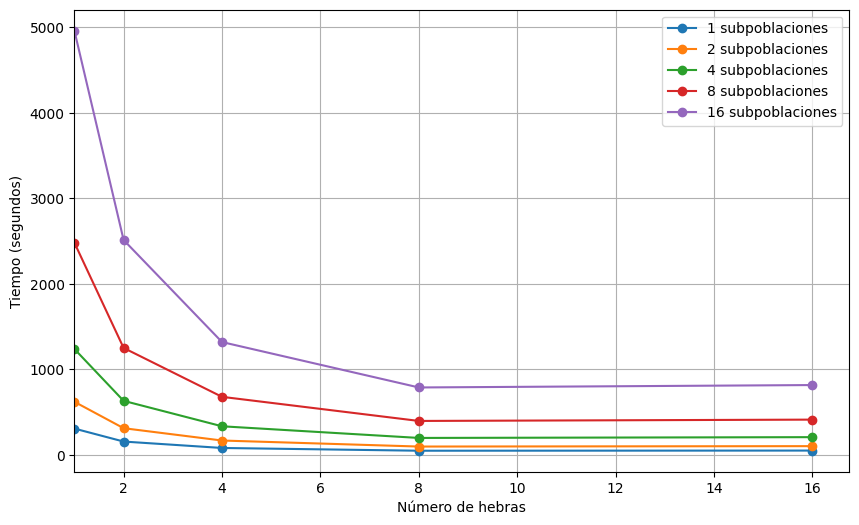
\includegraphics[width=0.8\textwidth]{imagenes/cap5/exploratory_subpopulations.png}
    \caption{Gráficas de ejecución de las pruebas variando el número de subpoblaciones y hebras.}
    \label{fig:exploratory_subpopulations}
\end{figure}

\begin{table}[ht]
    \centering
    \begin{tabular}{|c|ccccc|}
        \hline
        \multirow{2}{*}{\textbf{Hebras}} & \multicolumn{5}{c|}{\textbf{Subpoblaciones}}                                                      \\ \cline{2-6}
                                         & \textbf{1}                                   & \textbf{2} & \textbf{4} & \textbf{8} & \textbf{16} \\ \hline
        1                                & 309.43                                       & 622.63     & 1239.73    & 2481.89    & 4960.00     \\ \hline
        2                                & 157.79                                       & 313.86     & 633.66     & 1252.12    & 2513.72     \\ \hline
        4                                & 82.73                                        & 169.76     & 336.25     & 680.46     & 1320.66     \\ \hline
        8                                & 50.58                                        & 99.37      & 200.01     & 398.66     & 790.04      \\ \hline
        16                               & 52.32                                        & 104.06     & 209.17     & 414.11     & 818.17      \\ \hline
    \end{tabular}
    \caption{Tiempos de ejecución en segundos de las pruebas variando el número de subpoblaciones y hebras.}
    \label{tab:exploratory_subpopulations_times}
\end{table}

En la tabla \ref{tab:exploratory_populations_delta} se presentan los porcentajes de reducción del tiempo de ejecución respecto a la configuración base. En cada columna, la ejecución con una sola hebra y una sola subpoblación se toma como referencia (0\% de variación). Estos resultados permiten cuantificar de manera objetiva el beneficio relativo derivado del incremento del paralelismo y de la subdivisión de la población, proporcionando una base empírica para identificar configuraciones óptimas de ejecución.

\begin{table}[ht]
    \centering
    \begin{tabular}{|c|ccccc|}
        \hline
        \multirow{2}{*}{\textbf{Hebras}} & \multicolumn{5}{c|}{\textbf{Subpoblaciones}}                                                      \\ \cline{2-6}
                                         & \textbf{1}                                   & \textbf{2} & \textbf{4} & \textbf{8} & \textbf{16} \\ \hline
        1                                & 0.00                                         & 0.00       & 0.00       & 0.00       & 0.00        \\ \hline
        2                                & 49.01                                        & 49.59      & 48.89      & 49.55      & 49.32       \\ \hline
        4                                & 73.26                                        & 72.74      & 72.88      & 72.58      & 73.37       \\ \hline
        8                                & 83.65                                        & 84.04      & 83.87      & 83.94      & 84.07       \\ \hline
        16                               & 83.09                                        & 83.29      & 83.13      & 83.31      & 83.50       \\ \hline
    \end{tabular}
    \caption{Porcentaje de variación del tiempo de ejecución respecto a la configuración base para distintas combinaciones de hebras y subpoblaciones}
    \label{tab:exploratory_populations_delta}
\end{table}

Del análisis de esta tabla pueden extraerse varias conclusiones de interés para la definición de los parámetros en los experimentos posteriores. En primer lugar, se observa que, para un número fijo de hebras, la variación en el tiempo es prácticamente inexistente al modificar el número de subpoblaciones, lo que indica que el comportamiento es proporcional con independencia de este parámetro. En segundo lugar, el mayor beneficio en términos de reducción del tiempo de ejecución se obtiene al incrementar el número de hebras de 1 a 8, alcanzando valores en torno al 83--84\%. Sin embargo, al pasar de 8 a 16 hebras, los tiempos de ejecución se incrementan en todos los casos, lo que revela que se ha sobrepasado el punto de paralelismo óptimo para la arquitectura hardware utilizada. Este resultado sugiere que, en el entorno experimental considerado, el uso de más de 8 hebras no proporciona mejoras de rendimiento adicionales e, incluso, puede resultar contraproducente debido a la sobrecarga y la contención de recursos.

No obstante, se ha decidido mantener configuraciones con 16 hebras en los experimentos posteriores con el fin de analizar el comportamiento bajo condiciones de sobrecarga, dado que el objetivo del estudio trasciende la mera optimización de un caso específico y busca evaluar la escalabilidad y el rendimiento en un rango amplio de escenarios. En cuanto al número de subpoblaciones, se constata que con 16 subpoblaciones los tiempos de ejecución pueden alcanzar hasta 1 hora y 20 minutos en configuraciones con una única hebra, lo que resulta excesivo para los objetivos de este trabajo. Por el contrario, con 8 subpoblaciones se obtienen tiempos de ejecución más razonables, se alcanza un equilibrio adecuado entre eficiencia y aprovechamiento de recursos, y se garantiza una buena escalabilidad.

En consecuencia, se justifica la decisión metodológica de fijar el número de subpoblaciones en 8 para los experimentos posteriores, al representar un compromiso óptimo entre eficiencia, utilización de recursos y escalabilidad en el entorno analizado.

\subsection{Estudio del rendimiento al requerir más hebras de las disponibles}

En esta sección se presentan los resultados de las ejecuciones exploratorias realizadas para analizar el rendimiento de la aplicación al variar el número de procesos y hebras, incluyendo configuraciones que superan el límite físico de hebras de la CPU (16 hebras). El objetivo es comprender cómo afecta esta variación al tiempo de ejecución y al uso efectivo de la CPU, proporcionando una base para la selección de parámetros en estudios posteriores.

En la figura \ref{fig:exploratory_threads_limit_time} se muestra la evolución del tiempo de ejecución en función del número de hebras asignadas por proceso, para configuraciones que van desde 1 hasta 16 procesos, pero limitando el número máximo de hebras a 16.

\begin{figure}[ht]
    \centering
    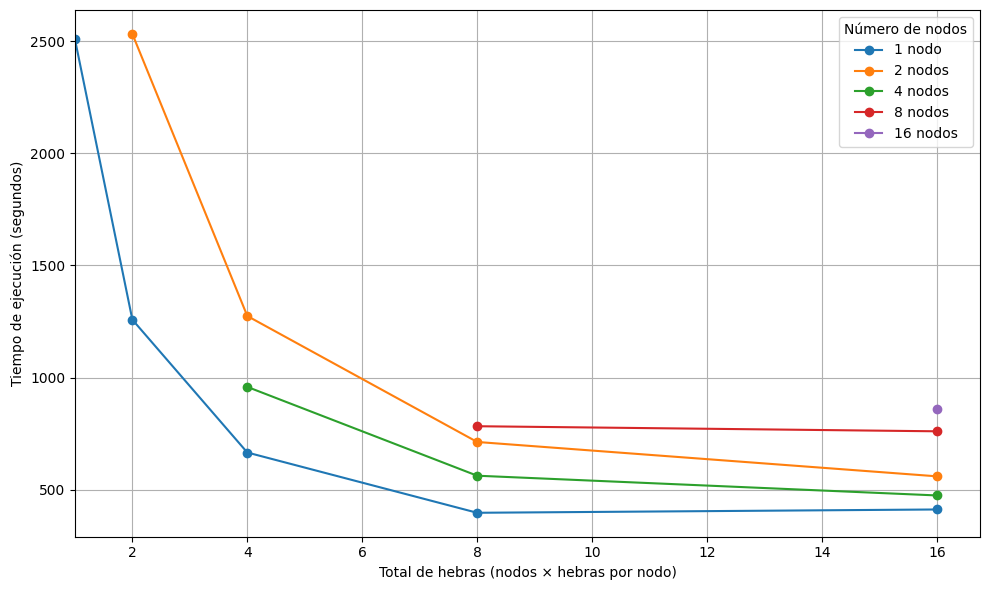
\includegraphics[width=0.8\textwidth]{imagenes/cap5/exploratory_threads_limit_time.png}
    \caption{Gráfica de tiempo de ejecución en función del número de hebras por proceso, con límite de 16 hebras.}
    \label{fig:exploratory_threads_limit_time}
\end{figure}

La figura \ref{fig:exploratory_threads_limit_cpu} muestra el porcentaje de uso total de CPU (donde 100\% equivale al uso completo de una hebra) para las distintas configuraciones de hebras por proceso analizadas.

\begin{figure}[ht]
    \centering
    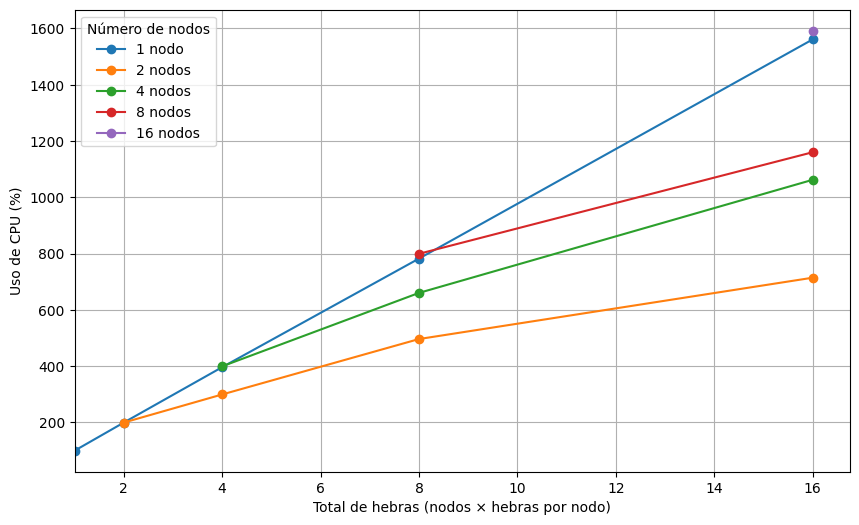
\includegraphics[width=0.8\textwidth]{imagenes/cap5/exploratory_threads_limit_cpu.png}
    \caption{Gráfica de uso de CPU en función del número de hebras por proceso, con límite de 16 hebras.}
    \label{fig:exploratory_threads_limit_cpu}
\end{figure}

Por otro lado, en la figura \ref{fig:exploratory_threads_no-limit_time} se presentan los resultados de las ejecuciones exploratorias sin límite en el número de hebras, permitiendo así evaluar el comportamiento del sistema al requerir más hebras de las disponibles.

\begin{figure}[ht]
    \centering
    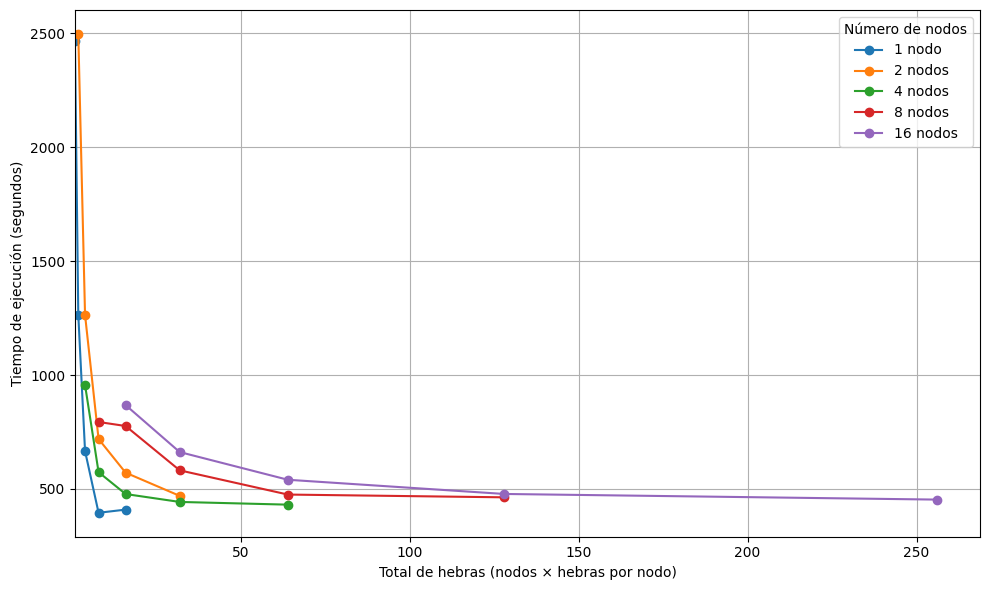
\includegraphics[width=0.8\textwidth]{imagenes/cap5/exploratory_threads_no-limit_time.png}
    \caption{Gráfica de tiempo de ejecución en función del número de hebras por proceso, sin límite en el número de hebras.}
    \label{fig:exploratory_threads_no-limit_time}
\end{figure}

La figura \ref{fig:exploratory_threads_no-limit_cpu} muestra el porcentaje de uso total de CPU para las distintas configuraciones de hebras por proceso sin límite, permitiendo observar cómo varía el aprovechamiento de los recursos en función del número total de hebras asignadas.

\begin{figure}[ht]
    \centering
    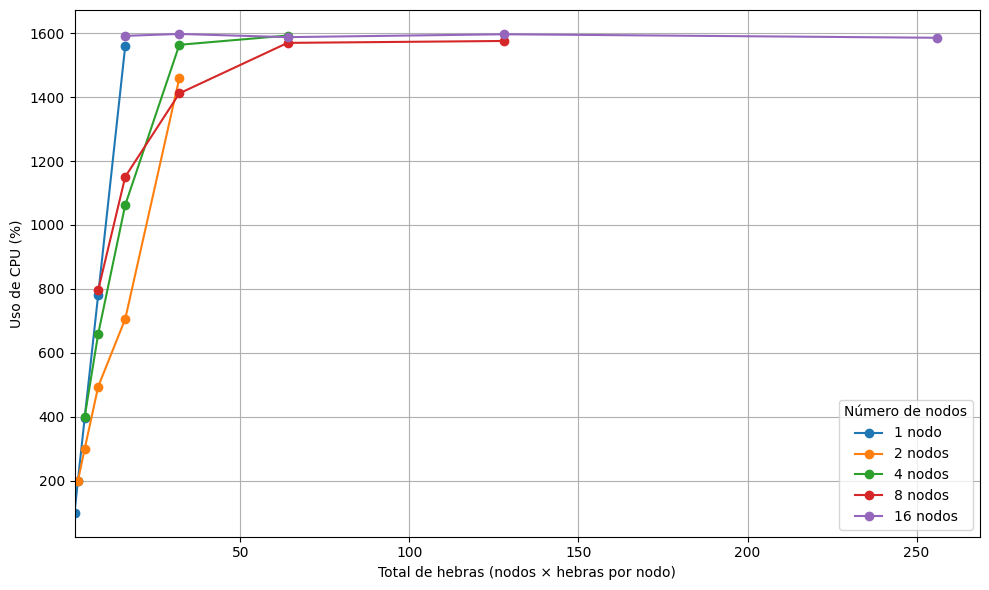
\includegraphics[width=0.8\textwidth]{imagenes/cap5/exploratory_threads_no-limit_cpu.png}
    \caption{Gráfica de uso de CPU en función del número de hebras por proceso, sin límite en el número de hebras.}
    \label{fig:exploratory_threads_no-limit_cpu}
\end{figure}

Las conclusiones que se pueden extraer de estas gráficas se pueden ver de manera más clara en la tabla \ref{tab:summary_nodes_threads_cpu}, donde se resumen los tiempos de ejecución y el uso de CPU para todas las combinaciones de procesos y hebras analizadas, tanto con límite como sin límite en el número de hebras.

\begin{table}[ht]
    \centering
    \small
    \setlength{\tabcolsep}{4pt}
    \renewcommand{\arraystretch}{1.1}
    \begin{tabular}{|c|c|c|c|c|}
        \hline
        \textbf{Procesos} & \textbf{Hebras}      & \textbf{Hebras}  & \textbf{Tiempo} & \textbf{Uso de}   \\
                          & \textbf{por proceso} & \textbf{totales} & \textbf{(s)}    & \textbf{CPU (\%)} \\
        \hline
        1                 & 8                    & 8                & 395.63          & 782               \\
        1                 & 16                   & 16               & 409.51          & 1561              \\
        4                 & 16                   & 64               & 431.30          & 1593              \\
        4                 & 8                    & 32               & 443.23          & 1564              \\
        16                & 16                   & 256              & 453.48          & 1586              \\
        8                 & 16                   & 128              & 463.45          & 1576              \\
        2                 & 16                   & 32               & 469.88          & 1460              \\
        8                 & 8                    & 64               & 475.59          & 1570              \\
        4                 & 4                    & 16               & 477.90          & 1063              \\
        16                & 8                    & 128              & 478.23          & 1597              \\
        16                & 4                    & 64               & 540.54          & 1588              \\
        2                 & 8                    & 16               & 571.65          & 706               \\
        4                 & 2                    & 8                & 573.94          & 659               \\
        8                 & 4                    & 32               & 581.91          & 1412              \\
        16                & 2                    & 32               & 662.10          & 1598              \\
        1                 & 4                    & 4                & 666.51          & 396               \\
        2                 & 4                    & 8                & 719.43          & 494               \\
        8                 & 2                    & 16               & 776.44          & 1151              \\
        8                 & 1                    & 8                & 794.09          & 796               \\
        16                & 1                    & 16               & 868.28          & 1592              \\
        4                 & 1                    & 4                & 956.38          & 399               \\
        2                 & 2                    & 4                & 1263.74         & 299               \\
        1                 & 2                    & 2                & 1264.94         & 199               \\
        1                 & 1                    & 1                & 2467.76         & 99                \\
        2                 & 1                    & 2                & 2497.06         & 199               \\
        \hline
    \end{tabular}
    \caption{Resumen de configuraciones de procesos, hebras y uso de CPU}
    \label{tab:summary_nodes_threads_cpu}
\end{table}

Los resultados muestran que el mejor rendimiento se alcanza empleando un menor número de procesos con un mayor número de hebras por proceso, siendo la configuración óptima la de un único proceso y ocho hebras. Aunque el límite físico de hebras de la CPU es de 16, se observa que, entre los diez mejores resultados, solo tres respetan este límite. En los demás casos, incrementar el número de hebras más allá de la capacidad física sigue proporcionando mejoras en el rendimiento, un comportamiento que, aunque inicialmente contraintuitivo, puede explicarse analizando el uso efectivo de la CPU.

El porcentaje de utilización de la CPU refleja el grado de aprovechamiento de las hebras disponibles: por ejemplo, con una hebra se alcanza un uso máximo de 100\%, con dos hebras el 200\%, y así sucesivamente hasta un máximo teórico de 1600\% (16 hebras $\times$ 100\%). En configuraciones de un único proceso, aumentar el número de hebras se traduce en un incremento proporcional del uso de CPU, lo que explica las mejoras de rendimiento observadas.

En contraste, cuando el número total de hebras se distribuye entre varios procesos, incluso si no se supera el límite físico de la CPU, el rendimiento no mejora de la misma manera. Esto se debe a la sobrecarga inherente a la gestión de múltiples procesos, que puede contrarrestar los beneficios de disponer de más hebras, haciendo que el uso efectivo de la CPU no alcance los valores esperados y resultando en un rendimiento inferior respecto a configuraciones monoproceso equivalentes. Por tanto, para configuraciones multiproceso es necesario incrementar el número de hebras más allá de la capacidad física de cada CPU para acercarse al uso máximo teórico, lo que explica por qué los mejores resultados se obtienen bajo estas condiciones.

\subsection{Estudio del rendimiento al utilizar la misma GPU en distintos procesos}

En esta sección se presentan los resultados de las ejecuciones exploratorias realizadas para analizar el rendimiento de la aplicación al variar el número de procesos y hebras, considerando dos enfoques distintos respecto al uso de la GPU: uno en el que se limita su uso a un único proceso y otro en el que se permite su uso en todos los procesos. El objetivo es comprender cómo afecta esta variación al tiempo de ejecución y al uso efectivo de la CPU, proporcionando una base para la selección de parámetros en estudios posteriores.

En la figura \ref{fig:exploratory_gpu_limit_time} se muestra la evolución del tiempo de ejecución en función del número de hebras asignadas por proceso, para configuraciones que van desde 1 hasta 16 procesos, limitando el uso de la GPU a un único proceso.

\begin{figure}[ht]
    \centering
    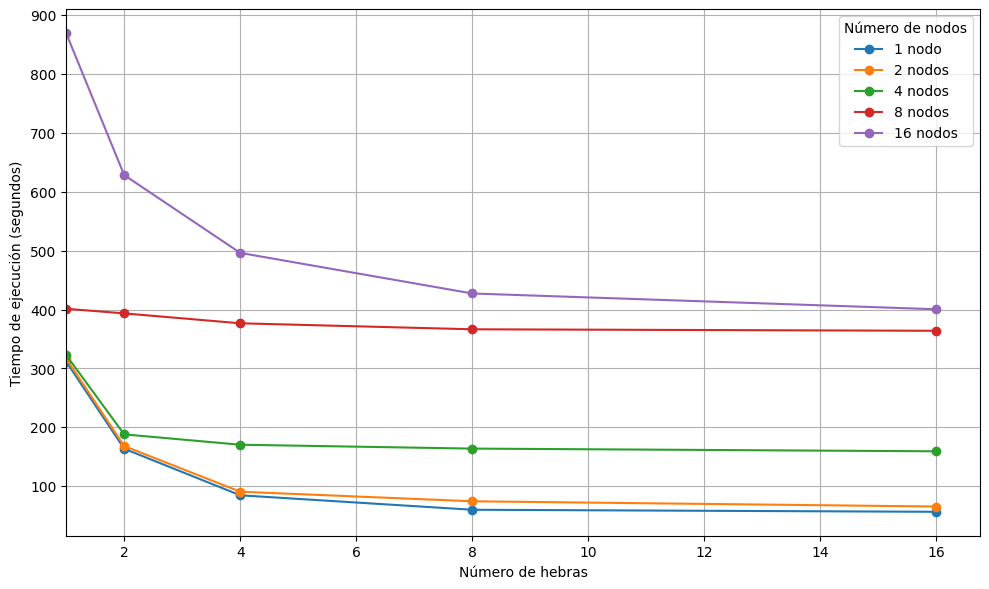
\includegraphics[width=0.8\textwidth]{imagenes/cap5/exploratory_gpu_limit_time.png}
    \caption{Gráfica de tiempo de ejecución en función del número de hebras por proceso, con la GPU limitada a un único proceso.}
    \label{fig:exploratory_gpu_limit_time}
\end{figure}

La figura \ref{fig:exploratory_gpu_no-limit_time} presenta los resultados de las ejecuciones exploratorias permitiendo el uso de la GPU en todos los procesos, evaluando así el comportamiento del sistema bajo esta configuración.

\begin{figure}[ht]
    \centering
    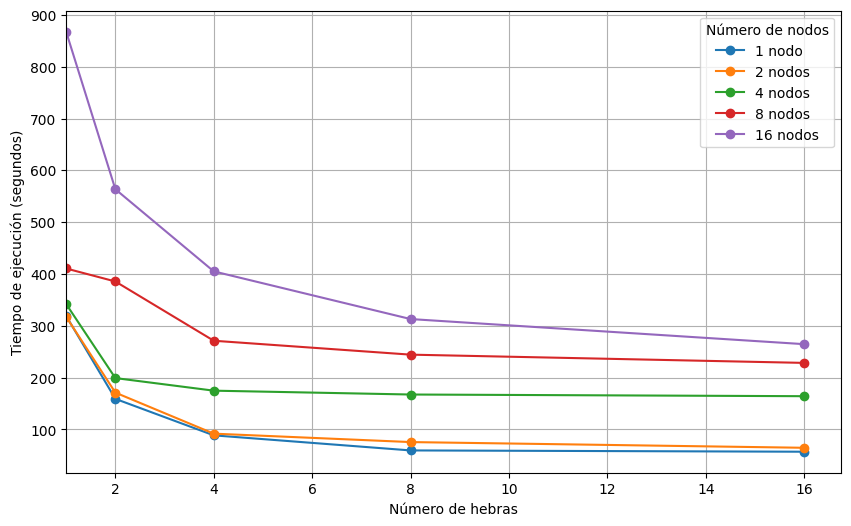
\includegraphics[width=0.8\textwidth]{imagenes/cap5/exploratory_gpu_no-limit_time.png}
    \caption{Gráfica de tiempo de ejecución en función del número de hebras por proceso, permitiendo el uso de la GPU en todos los procesos.}
    \label{fig:exploratory_gpu_no-limit_time}
\end{figure}

Las conclusiones que se pueden extraer de estas gráficas se pueden ver de manera más clara en la tabla \ref{tab:summary_nodes_threads_gpu}, donde se resumen los tiempos de ejecución para todas las combinaciones de procesos y hebras analizadas, tanto con la GPU limitada a un proceso como permitiendo su uso en todos los procesos.

\begin{table}[ht]
    \centering
    \scriptsize
    \setlength{\tabcolsep}{2pt}
    \renewcommand{\arraystretch}{1.1}
    \begin{tabular}{|c|c|c|c|c|}
        \hline
        \textbf{Procesos} & \textbf{Hebras} & \textbf{GPU 1 proceso (s)} & \textbf{GPU todos (s)} & \textbf{Var. (\%)} \\
        \hline
        1                 & 1               & 311.68                     & 319.01                 & 2.35               \\
        1                 & 2               & 163.59                     & 158.94                 & -2.84              \\
        1                 & 4               & 84.49                      & 88.52                  & 4.77               \\
        1                 & 8               & 59.91                      & 59.41                  & -0.83              \\
        1                 & 16              & 56.45                      & 56.91                  & 0.81               \\
        2                 & 1               & 316.92                     & 317.35                 & 0.14               \\
        2                 & 2               & 168.14                     & 170.99                 & 1.70               \\
        2                 & 4               & 90.58                      & 91.78                  & 1.32               \\
        2                 & 8               & 74.30                      & 75.53                  & 1.66               \\
        2                 & 16              & 65.40                      & 64.51                  & -1.36              \\
        4                 & 1               & 322.77                     & 341.95                 & 5.94               \\
        4                 & 2               & 187.98                     & 199.04                 & 5.88               \\
        4                 & 4               & 170.38                     & 174.74                 & 2.56               \\
        4                 & 8               & 163.80                     & 167.31                 & 2.14               \\
        4                 & 16              & 159.22                     & 164.07                 & 3.05               \\
        8                 & 1               & 401.33                     & 410.54                 & 2.29               \\
        8                 & 2               & 393.50                     & 385.47                 & -2.04              \\
        8                 & 4               & 376.68                     & 271.10                 & -28.03             \\
        8                 & 8               & 366.47                     & 244.26                 & -33.35             \\
        8                 & 16              & 363.94                     & 228.34                 & -37.26             \\
        16                & 1               & 869.40                     & 867.50                 & -0.22              \\
        16                & 2               & 628.49                     & 563.51                 & -10.34             \\
        16                & 4               & 496.28                     & 404.98                 & -18.40             \\
        16                & 8               & 427.30                     & 312.94                 & -26.76             \\
        16                & 16              & 400.48                     & 264.49                 & -33.96             \\
        \hline
    \end{tabular}
    \caption{Resumen de tiempos de ejecución para distintas combinaciones de procesos y hebras, comparando el uso de la GPU limitada a un proceso frente a su uso en todos los procesos.}
    \label{tab:summary_nodes_threads_gpu}
\end{table}

Para configuraciones con pocos procesos (1, 2 o 4), la diferencia entre utilizar la GPU en un único proceso o en todos los procesos resulta pequeña y variable. Las variaciones porcentuales oscilan entre valores positivos y negativos, pero en general se mantienen por debajo del 6\%. Esto indica que, en estos escenarios, no existe una ventaja clara ni consistente de emplear la GPU de forma compartida en todos los procesos.

A partir de 8 procesos, la ejecución con la GPU disponible en todos los procesos comienza a mostrar mejoras significativas, especialmente al incrementar el número de hebras. Por ejemplo, con 8 procesos y 16 hebras se observa una reducción del tiempo de ejecución del 37.26\%, mientras que con 16 procesos y 16 hebras la mejora alcanza el 33.96\%. Estas diferencias son consistentes y tienden a aumentar conforme crece el número de procesos y hebras.

En configuraciones con un número elevado de procesos y hebras, la opción de permitir el acceso a la GPU en todos los procesos se presenta como claramente superior, ya que maximiza el aprovechamiento de la capacidad de cómputo distribuido y reduce de manera significativa los tiempos de ejecución.

En resumen, para experimentos pequeños o con pocos procesos ambas opciones resultan comparables. Sin embargo, en experimentos de mayor escala y con configuraciones que involucran un alto número de procesos y hebras, la estrategia más eficiente y recomendable es habilitar el uso de la GPU en todos los procesos.

\subsection{Análisis de los experimentos preliminares}

A partir de los resultados obtenidos, se recomienda fijar el número de subpoblaciones en 8, ya que este valor representa un equilibrio óptimo entre eficiencia, utilización de recursos y escalabilidad en el entorno analizado.

En cuanto al número de hebras, los datos muestran que imponer un límite estricto puede restringir el aprovechamiento total de los recursos, especialmente en configuraciones multiproceso. Por ello, se recomienda no limitar el número de hebras, permitiendo que el sistema utilice tantas como sean necesarias para maximizar el rendimiento.

Respecto al uso de la GPU, los experimentos indican que en configuraciones pequeñas las diferencias entre habilitarla en todos los procesos o solo en uno son mínimas. Sin embargo, en escenarios de mayor escala, habilitar su uso en todos los procesos aporta mejoras sustanciales en el tiempo de ejecución y en la eficiencia global. Por tanto, se establece como criterio general que la GPU esté disponible en todos los procesos.

En conjunto, estas decisiones proporcionan una base sólida y coherente para el diseño de los experimentos posteriores, asegurando que se exploten al máximo los recursos disponibles sin comprometer la comparabilidad de los resultados.

\section{Pruebas monoproceso}

\subsection{Ejecución en Ubuntu en nativo}

\subsubsection{CPU}

En la figura \ref{fig:single-node_ubuntu_cpu_native_time} se muestra el tiempo de ejecución para la configuración de CPU en un único proceso con Ubuntu nativo.

\begin{figure}[H]
    \centering
    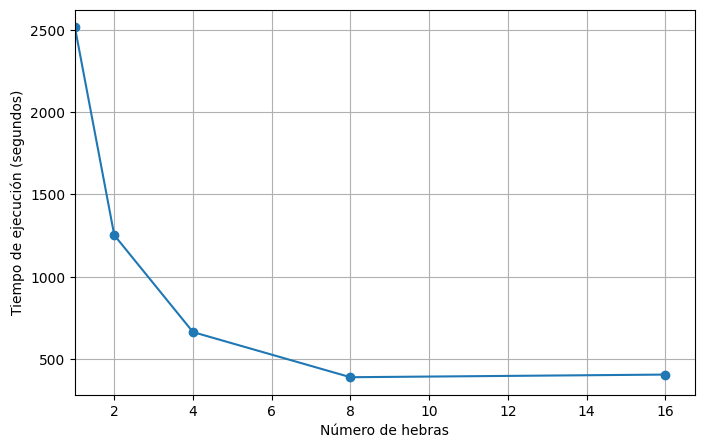
\includegraphics[width=0.8\textwidth]{imagenes/cap5/single-node_ubuntu_cpu_native_time.png}
    \caption{Tiempo de ejecución en función del número de hebras en Ubuntu nativo (CPU).}
    \label{fig:single-node_ubuntu_cpu_native_time}
\end{figure}

En la tabla \ref{tab:single-node_ubuntu_cpu_native} se presentan los tiempos de ejecución y la variación porcentual respecto a una hebra.

\begin{table}[ht]
    \centering
    \begin{tabular}{|c|c|c|}
        \hline
        \textbf{Hebras} & \textbf{Tiempo (s)} & \textbf{$\Delta$\% vs 1 hebra} \\
        \hline
        1               & 2515.21             & 0.00                           \\
        2               & 1253.18             & -50.18                         \\
        4               & 664.69              & -73.57                         \\
        8               & 390.72              & -84.47                         \\
        16              & 406.76              & -83.83                         \\
        \hline
    \end{tabular}
    \caption{Tiempos de ejecución y variación porcentual respecto a una hebra en Ubuntu nativo (CPU).}
    \label{tab:single-node_ubuntu_cpu_native}
\end{table}

El tiempo de ejecución disminuye drásticamente al aumentar el número de hebras, especialmente en el rango de $1$ a $8$ hebras. Con $2$ hebras, el tiempo se reduce prácticamente a la mitad ($-50.18\%$), y con $4$ hebras, a casi una cuarta parte del tiempo original ($-73.57\%$). El mayor beneficio se observa al pasar de $4$ a $8$ hebras, alcanzando una reducción del $84.47\%$ respecto a una hebra. Sin embargo, al incrementar a $16$ hebras, el tiempo de ejecución es ligeramente superior al obtenido con $8$ hebras, lo que sugiere la aparición de saturación o sobrecarga en el sistema. Por tanto, el óptimo se alcanza con $8$ hebras, coincidiendo con el número de núcleos físicos disponibles en el sistema.

En la figura \ref{fig:single-node_ubuntu_cpu_native_cpu} se muestra el porcentaje de uso de CPU en función del número de hebras.

\begin{figure}[H]
    \centering
    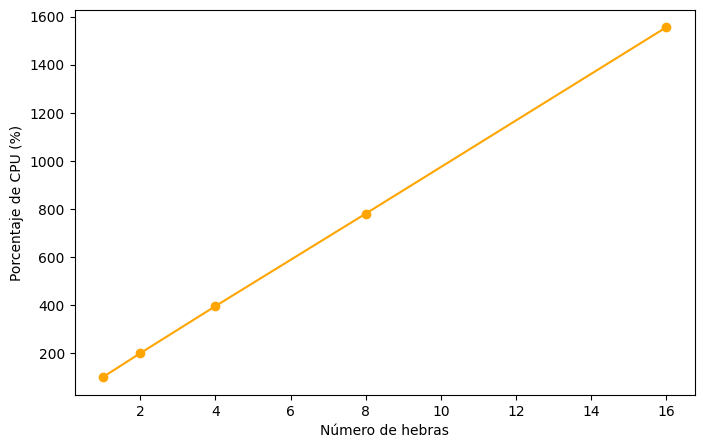
\includegraphics[width=0.8\textwidth]{imagenes/cap5/single-node_ubuntu_cpu_native_cpu.png}
    \caption{Uso de CPU en función del número de hebras en Ubuntu nativo (CPU).}
    \label{fig:single-node_ubuntu_cpu_native_cpu}
\end{figure}

La tabla \ref{tab:single-node_ubuntu_cpu_native_cpu} muestra el porcentaje de uso de CPU alcanzado para cada número de hebras, el máximo teórico posible (calculado como número de hebras por 100\%), y la eficiencia relativa obtenida.

\begin{table}[ht]
    \centering
    \begin{tabular}{|c|c|c|c|}
        \hline
        \textbf{Hebras} & \textbf{CPU (\%)} & \textbf{Max posible CPU (\%)} & \textbf{Efic. CPU (\%)} \\
        \hline
        1               & 99.00             & 100.00                        & 99.00                   \\
        2               & 199.00            & 200.00                        & 99.50                   \\
        4               & 395.00            & 400.00                        & 98.75                   \\
        8               & 780.00            & 800.00                        & 97.50                   \\
        16              & 1556.00           & 1600.00                       & 97.25                   \\
        \hline
    \end{tabular}
    \caption{Porcentaje de uso de CPU y eficiencia en función del número de hebras en Ubuntu nativo (CPU).}
    \label{tab:single-node_ubuntu_cpu_native_cpu}
\end{table}

El uso de CPU aumenta de manera casi lineal conforme se incrementa el número de hebras, lo que evidencia un excelente escalado del paralelismo en la ejecución. La eficiencia de uso de la CPU se mantiene muy elevada en todos los casos, superando el $97\%$, lo que indica que prácticamente se está aprovechando todo el potencial de cómputo disponible. Aunque la eficiencia disminuye ligeramente al aumentar el número de hebras (desde un máximo del $99\%$ hasta un mínimo del $97.25\%$), esta reducción es mínima y esperable, ya que responde a la sobrecarga asociada a la gestión de un mayor número de hilos y a posibles contenciones internas. En conjunto, el sistema demuestra un escalado eficiente hasta $16$ hebras, con una pérdida de eficiencia muy reducida.

Estos resultados evidencian que el entorno monoproceso nativo en Ubuntu gestiona eficazmente el paralelismo y aprovecha bien los recursos de la CPU, mostrando un buen escalado del rendimiento al aumentar el número de hebras.

\subsubsection{CPU + GPU}

En la figura \ref{fig:single-node_ubuntu__gpu_native_time} se muestra el tiempo de ejecución para la configuración de CPU + GPU en un único proceso con Ubuntu nativo.

\begin{figure}[H]
    \centering
    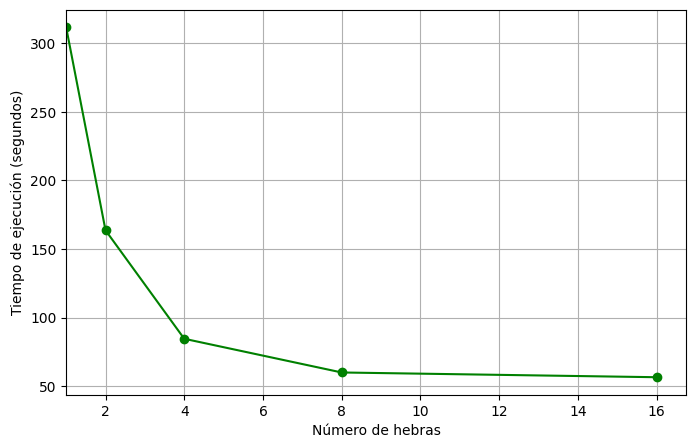
\includegraphics[width=0.8\textwidth]{imagenes/cap5/single-node_ubuntu_gpu_native_time.png}
    \caption{Tiempo de ejecución en función del número de hebras en Ubuntu nativo (CPU + GPU).}
    \label{fig:single-node_ubuntu__gpu_native_time}
\end{figure}

En la tabla \ref{tab:single-node_ubuntu_gpu_native} se presentan los tiempos de ejecución y la variación porcentual respecto a una hebra.

\begin{table}[ht]
    \centering
    \begin{tabular}{|c|c|c|}
        \hline
        \textbf{Hebras} & \textbf{Tiempo (s)} & \textbf{$\Delta$\% vs 1 hebra} \\
        \hline
        1.00            & 311.68              & 0.00                           \\
        2.00            & 163.59              & -47.51                         \\
        4.00            & 84.49               & -72.89                         \\
        8.00            & 59.91               & -80.78                         \\
        16.00           & 56.45               & -81.89                         \\
        \hline
    \end{tabular}
    \caption{Tiempos de ejecución y variación porcentual respecto a una hebra en Ubuntu nativo (CPU + GPU).}
    \label{tab:single-node_ubuntu_gpu_native}
\end{table}

El análisis de los resultados muestra que el tiempo de ejecución disminuye de forma significativa al incrementar el número de hebras, especialmente en el rango de $1$ a $4$ hebras, donde se alcanza una reducción del $72.89\%$. La mayor ganancia relativa se produce al pasar de $1$ a $2$ hebras ($-47.51\%$) y de $2$ a $4$ hebras ($-25.38\%$ adicional). Sin embargo, a partir de $8$ hebras, la mejora es marginal: el tiempo de ejecución solo disminuye de $59.91\,s$ a $56.45\,s$ al pasar de $8$ a $16$ hebras, lo que supone apenas un $1.11\%$ adicional. Esto indica que el sistema alcanza un punto óptimo de rendimiento con $8$ hebras, y que a partir de ese valor se observa una saturación en la eficiencia de la paralelización. En conjunto, la combinación CPU + GPU proporciona una aceleración notable, pero la eficiencia se estabiliza a partir de cierto número de hebras, reflejando el límite práctico de paralelismo efectivo en el entorno analizado.

\subsubsection{Comparativa CPU vs CPU + GPU}

En la figura \ref{fig:single-node_ubuntu_cpu_vs_gpu_native_time} se muestra una comparativa del tiempo de ejecución entre las configuraciones de CPU y CPU + GPU en un único proceso con Ubuntu nativo.

\begin{figure}[H]
    \centering
    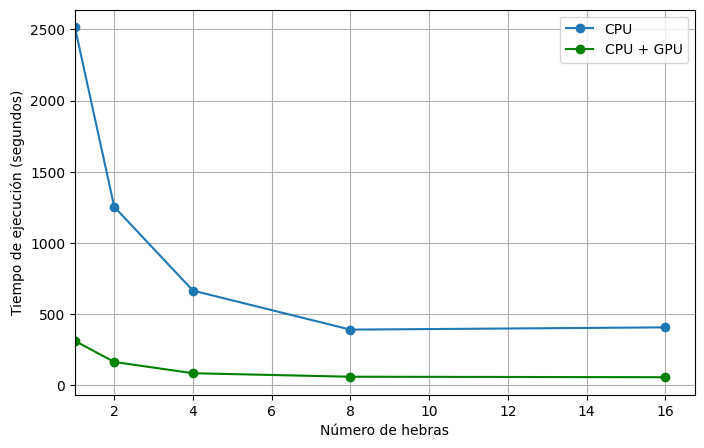
\includegraphics[width=0.8\textwidth]{imagenes/cap5/single-node_ubuntu_cpu_vs_gpu_native_time.png}
    \caption{Comparativa de tiempo de ejecución entre CPU y CPU + GPU en función del número de hebras en Ubuntu nativo.}
    \label{fig:single-node_ubuntu_cpu_vs_gpu_native_time}
\end{figure}

En la tabla \ref{tab:single-node_ubuntu_cpu_vs_gpu_native} se presentan los tiempos de ejecución para ambas configuraciones y la variación porcentual entre ellas.

\begin{table}[ht]
    \centering
    \begin{tabular}{|c|c|c|c|}
        \hline
        \textbf{Hebras} & \textbf{Tiempo CPU (s)} & \textbf{Tiempo CPU+GPU (s)} & \textbf{Var. (\%)} \\
        \hline
        1               & 2515.21                 & 311.68                      & -87.61             \\
        2               & 1253.18                 & 163.59                      & -86.95             \\
        4               & 664.69                  & 84.49                       & -87.29             \\
        8               & 390.72                  & 59.91                       & -84.67             \\
        16              & 406.76                  & 56.45                       & -86.12             \\
        \hline
    \end{tabular}
    \caption{Comparativa de tiempos de ejecución y variación porcentual entre CPU y CPU+GPU en Ubuntu nativo.}
    \label{tab:single-node_ubuntu_cpu_vs_gpu_native}
\end{table}

El análisis de los resultados muestra que el uso de GPU reduce el tiempo de ejecución entre un $84\%$ y un $88\%$ respecto a la ejecución únicamente en CPU, independientemente del número de hebras empleadas. La mejora relativa se mantiene estable al aumentar el paralelismo, lo que indica que la GPU aporta un beneficio constante y no dependiente del número de hilos de CPU utilizados. Además, mientras que en la configuración solo CPU el tiempo de ejecución deja de mejorar al pasar de $8$ a $16$ hebras (e incluso empeora ligeramente), en la configuración CPU+GPU la mejora es marginal pero consistente. En conjunto, la incorporación de GPU resulta altamente beneficiosa, acelerando el procesamiento en torno al $85\%$ en todos los escenarios analizados.

\subsection{Ejecución en contenedores de Ubuntu}
\subsubsection{CPU}

En la figura \ref{fig:single-node_ubuntu_docker_time} se muestra el tiempo de ejecución para la configuración de CPU en un único proceso con contenedores de Ubuntu.

\begin{figure}[H]
    \centering
    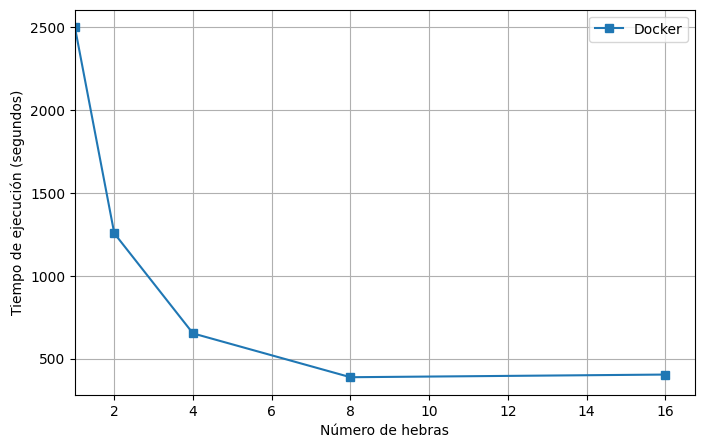
\includegraphics[width=0.8\textwidth]{imagenes/cap5/single-node_ubuntu_docker_time.png}
    \caption{Tiempo de ejecución en un único proceso con contenedores de Ubuntu (CPU).}
    \label{fig:single-node_ubuntu_docker_time}
\end{figure}

En la tabla \ref{tab:single-node_ubuntu_docker} se presentan los tiempos de ejecución y la variación porcentual respecto a una hebra.

\begin{table}[ht]
    \centering
    \begin{tabular}{|c|c|c|}
        \hline
        \textbf{Hebras} & \textbf{Tiempo (s)} & \textbf{$\Delta$\% vs 1 hebra} \\
        \hline
        1               & 2499.09             & 0.00                           \\
        2               & 1255.95             & -49.74                         \\
        4               & 652.33              & -73.90                         \\
        8               & 388.04              & -84.47                         \\
        16              & 404.09              & -83.83                         \\
        \hline
    \end{tabular}
    \caption{Tiempos de ejecución y variación porcentual respecto a una hebra en contenedores de Ubuntu (CPU).}
    \label{tab:single-node_ubuntu_docker}
\end{table}

El tiempo de ejecución disminuye significativamente al aumentar el número de hebras, especialmente al pasar de 1 a 8 hebras, donde la reducción alcanza el 84.47\%.

La mayor ganancia relativa se obtiene al pasar de 1 a 2 hebras (-49.74\%) y de 2 a 4 hebras (-48.16\% adicional), mostrando una buena escalabilidad inicial.

A partir de 8 hebras, la mejora se estabiliza y el rendimiento apenas varía, e incluso con 16 hebras el tiempo de ejecución es ligeramente superior al de 8 hebras, lo que indica que se alcanza un límite de paralelización eficiente.

Estos resultados sugieren que, en este entorno, el uso de más de 8 hebras no aporta beneficios significativos y puede incluso generar sobrecarga, por lo que 8 hebras representa el punto óptimo de eficiencia para la ejecución en contenedores de Ubuntu con CPU.

En la figura \ref{fig:single-node_ubuntu_podman_time} se muestra el tiempo de ejecución para la configuración de CPU en un único proceso con contenedores de Ubuntu gestionados por \textit{Podman}.

\begin{figure}[H]
    \centering
    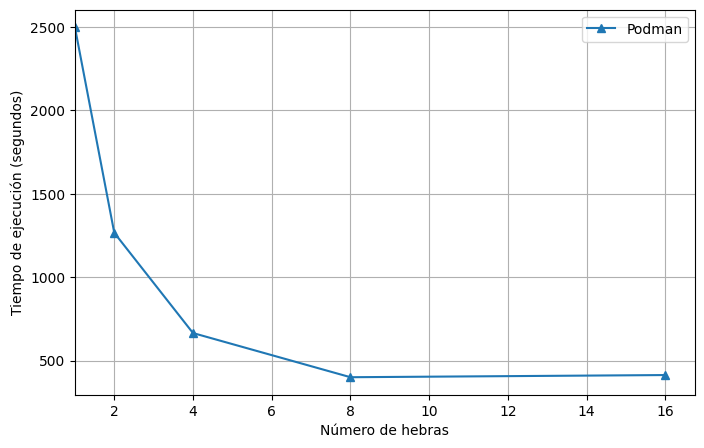
\includegraphics[width=0.8\textwidth]{imagenes/cap5/single-node_ubuntu_podman_time.png}
    \caption{Tiempo de ejecución en un único proceso con contenedores de Ubuntu gestionados por \textit{Podman} (CPU).}
    \label{fig:single-node_ubuntu_podman_time}
\end{figure}

En la tabla \ref{tab:single-node_ubuntu_podman} se presentan los tiempos de ejecución y la variación porcentual respecto a una hebra.

\begin{table}[ht]
    \centering
    \begin{tabular}{|c|c|c|}
        \hline
        \textbf{Hebras} & \textbf{Tiempo (s)} & \textbf{$\Delta$\% vs 1 hebra} \\
        \hline
        1               & 2499.16             & 0.00                           \\
        2               & 1266.51             & -49.32                         \\
        4               & 665.38              & -73.38                         \\
        8               & 400.51              & -83.97                         \\
        16              & 413.53              & -83.45                         \\
        \hline
    \end{tabular}
    \caption{Tiempos de ejecución y variación porcentual respecto a una hebra en contenedores de Ubuntu gestionados por \textit{Podman} (CPU).}
    \label{tab:single-node_ubuntu_podman}
\end{table}

El tiempo de ejecución disminuye de forma considerable al aumentar el número de hebras, especialmente entre 1 y 8 hebras, donde la reducción alcanza el 83.97\%.

La mayor mejora relativa se observa al pasar de 1 a 2 hebras (-49.32\%) y de 2 a 4 hebras (-47.97\% adicional), lo que indica una buena escalabilidad inicial.

A partir de 8 hebras, la reducción en el tiempo de ejecución se estabiliza y el beneficio adicional es mínimo; con 16 hebras, el tiempo incluso aumenta ligeramente respecto a 8 hebras, lo que sugiere que se alcanza el límite de paralelización eficiente.

Estos resultados muestran que, en este entorno con \textit{Podman} y CPU, el uso óptimo se encuentra en torno a 8 hebras, ya que aumentar más allá de este valor no aporta mejoras significativas y puede generar sobrecarga.

\subsubsection{CPU + GPU}

En la figura \ref{fig:single-node_ubuntu_docker_gpu_time} se muestra el tiempo de ejecución para la configuración de CPU + GPU en un único proceso con contenedores de Ubuntu.

\begin{figure}[H]
    \centering
    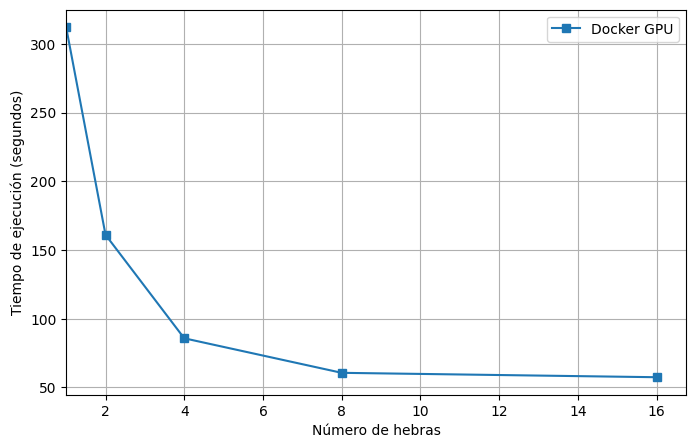
\includegraphics[width=0.8\textwidth]{imagenes/cap5/single-node_ubuntu_docker_gpu_time.png}
    \caption{Tiempo de ejecución en un único proceso con contenedores de Ubuntu (CPU + GPU).}
    \label{fig:single-node_ubuntu_docker_gpu_time}
\end{figure}

En la tabla \ref{tab:single-node_ubuntu_docker_gpu} se presentan los tiempos de ejecución y la variación porcentual respecto a una hebra.

\begin{table}[ht]
    \centering
    \begin{tabular}{|c|c|c|}
        \hline
        \textbf{Hebras} & \textbf{Tiempo (s)} & \textbf{$\Delta$\% vs 1 hebra} \\
        \hline
        1               & 312.18              & 0.00                           \\
        2               & 161.10              & -48.40                         \\
        4               & 85.78               & -72.52                         \\
        8               & 60.65               & -80.57                         \\
        16              & 57.45               & -81.60                         \\
        \hline
    \end{tabular}
    \caption{Tiempos de ejecución y variación porcentual respecto a una hebra en contenedores de Ubuntu (CPU + GPU).}
    \label{tab:single-node_ubuntu_docker_gpu}
\end{table}

El uso combinado de CPU y GPU en contenedores de Ubuntu permite una variación muy significativa en los tiempos de ejecución al aumentar el número de hebras, alcanzando una disminución del 81.60\% con 16 hebras respecto a la ejecución con una sola hebra.

La mayor ganancia relativa se observa al pasar de 1 a 2 hebras (-48.40\%) y de 2 a 4 hebras (-24.12\% adicional), lo que indica una buena escalabilidad inicial.

A partir de 8 hebras, la mejora se estabiliza y el beneficio adicional es marginal; el tiempo de ejecución con 16 hebras es solo ligeramente menor que con 8 hebras.

Estos resultados muestran que, en este entorno, la combinación de CPU y GPU permite aprovechar eficientemente el paralelismo hasta 8 hebras, siendo el punto óptimo de eficiencia, ya que aumentar más allá de este valor aporta mejoras muy pequeñas.

En la figura \ref{fig:single-node_ubuntu_podman_gpu_time} se muestra el tiempo de ejecución para la configuración de CPU + GPU en un único proceso con contenedores de Ubuntu gestionados por \textit{Podman}.

\begin{figure}[H]
    \centering
    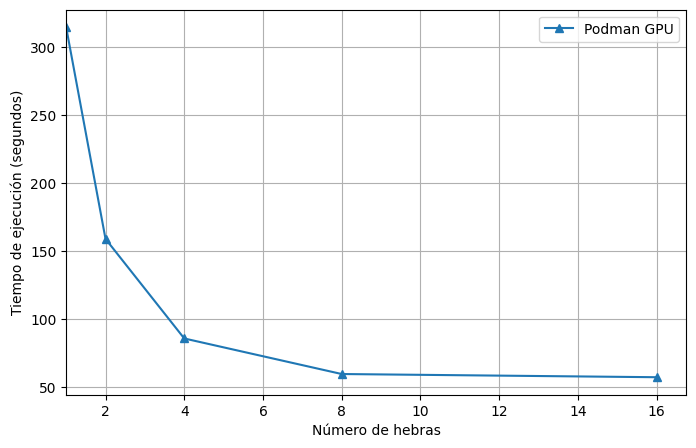
\includegraphics[width=0.8\textwidth]{imagenes/cap5/single-node_ubuntu_podman_gpu_time.png}
    \caption{Tiempo de ejecución en un único proceso con contenedores de Ubuntu gestionados por \textit{Podman} (CPU + GPU).}
    \label{fig:single-node_ubuntu_podman_gpu_time}
\end{figure}

En la tabla \ref{tab:single-node_ubuntu_podman_gpu} se presentan los tiempos de ejecución y la variación porcentual respecto a una hebra.

\begin{table}[ht]
    \centering
    \begin{tabular}{|c|c|c|}
        \hline
        \textbf{Hebras} & \textbf{Tiempo (s)} & \textbf{$\Delta$\% vs 1 hebra} \\
        \hline
        1               & 314.51              & 0.00                           \\
        2               & 158.84              & -49.50                         \\
        4               & 85.62               & -72.78                         \\
        8               & 59.47               & -81.09                         \\
        16              & 57.12               & -81.84                         \\
        \hline
    \end{tabular}
    \caption{Tiempos de ejecución y variación porcentual respecto a una hebra en contenedores de Ubuntu gestionados por \textit{Podman} (CPU + GPU).}
    \label{tab:single-node_ubuntu_podman_gpu}
\end{table}

El tiempo de ejecución disminuye drásticamente al aumentar el número de hebras, alcanzando una reducción del 81.84\% con 16 hebras respecto a la ejecución con una sola hebra.

La mayor mejora relativa se observa al pasar de 1 a 2 hebras (-49.50\%) y de 2 a 4 hebras (-23.28\% adicional), lo que indica una excelente escalabilidad inicial.

A partir de 8 hebras, la reducción en el tiempo de ejecución se estabiliza y el beneficio adicional es muy pequeño; el tiempo con 16 hebras es solo ligeramente menor que con 8 hebras.

Estos resultados muestran que, en este entorno con \textit{Podman} y CPU+GPU, el uso óptimo se encuentra en torno a 8 hebras, ya que aumentar más allá de este valor no aporta mejoras significativas y puede generar sobrecarga.

\subsubsection{Comparativa contenedores vs nativo}

En la figura \ref{fig:single-node_ubuntu_container_vs_native_time} se muestra una comparativa del tiempo de ejecución entre las configuraciones nativas y en contenedores de Ubuntu para CPU.

\begin{figure}[H]
    \centering
    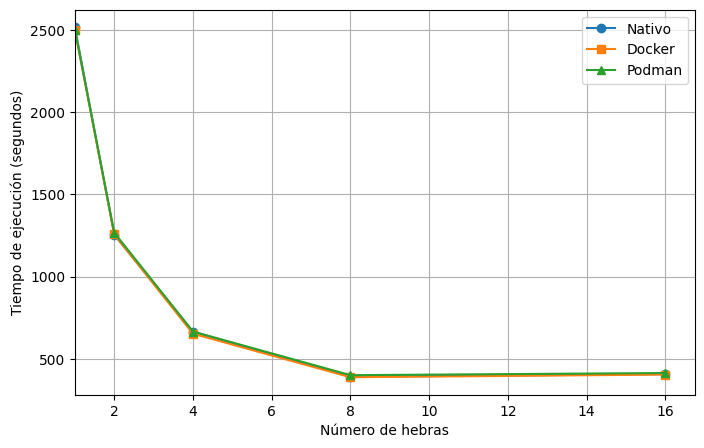
\includegraphics[width=0.8\textwidth]{imagenes/cap5/single-node_ubuntu_container_vs_native_time.png}
    \caption{Comparativa de tiempo de ejecución entre nativo y contenedores de Ubuntu en función del número de hebras, para CPU.}
    \label{fig:single-node_ubuntu_container_vs_native_time}
\end{figure}

En la tabla \ref{tab:single-node_ubuntu_container_vs_native} se presentan los tiempos de ejecución para ambas configuraciones y la variación porcentual entre ellas.

\begin{table}[ht]
    \centering
    \begin{tabular}{|c|c|c|c|c|c|}
        \hline
        \textbf{Hebras} & \textbf{Nativo (s)} & \textbf{\textit{Docker} (s)} & \textbf{\textit{Docker} $\Delta$\%} & \textbf{\textit{Podman} (s)} & \textbf{\textit{Podman} $\Delta$\%} \\
        \hline
        1.00            & 2515.21             & 2499.09                      & -0.64                               & 2499.16                      & -0.64                               \\
        2.00            & 1253.18             & 1255.95                      & 0.22                                & 1266.51                      & 1.06                                \\
        4.00            & 664.69              & 652.33                       & -1.86                               & 665.38                       & 0.10                                \\
        8.00            & 390.72              & 388.04                       & -0.69                               & 400.51                       & 2.51                                \\
        16.00           & 406.76              & 404.09                       & -0.66                               & 413.53                       & 1.66                                \\
        \hline
    \end{tabular}
    \caption{Comparativa de tiempos de ejecución entre nativo, \textit{Docker} y \textit{Podman} en función del número de hebras y variación porcentual respecto a nativo (CPU, monoproceso).}
    \label{tab:single-node_ubuntu_container_vs_native}
\end{table}

La tabla compara los tiempos de ejecución entre los entornos nativo, \textit{Docker} y \textit{Podman} en un escenario monoproceso utilizando únicamente CPU y diferentes números de hebras, mostrando además la variación porcentual de los contenedores respecto al entorno nativo. Con una hebra, tanto \textit{Docker} como \textit{Podman} presentan tiempos de ejecución ligeramente inferiores al nativo, con una reducción del 0.64\%, lo que indica que la sobrecarga de los contenedores es prácticamente inexistente en este caso. Al aumentar a dos hebras, \textit{Docker} muestra un incremento mínimo del 0.22\% y \textit{Podman} del 1.06\%, lo que sugiere que la eficiencia de los contenedores se mantiene muy próxima a la del entorno nativo. Con cuatro hebras, \textit{Docker} logra una mejora del 1.86\% respecto al nativo, mientras que \textit{Podman} se mantiene prácticamente igual, lo que podría estar relacionado con pequeñas diferencias en la gestión de recursos internos. Al incrementar el número de hebras a ocho y dieciséis, las diferencias siguen siendo muy reducidas, con \textit{Docker} mostrando ligeras mejoras y \textit{Podman} presentando incrementos moderados, pero siempre dentro de un margen muy estrecho. En conjunto, estos resultados evidencian que el uso de contenedores en un entorno monoproceso y CPU no introduce penalizaciones significativas en el rendimiento y, en algunos casos, puede incluso aportar pequeñas mejoras, confirmando la viabilidad de \textit{Docker} y \textit{Podman} para la ejecución eficiente de aplicaciones paralelas en este tipo de escenarios.

La figura \ref{fig:single-node_ubuntu_container_vs_native_gpu_time} muestra una comparativa del tiempo de ejecución entre las configuraciones nativas y en contenedores de Ubuntu para CPU + GPU.

\begin{figure}[H]
    \centering
    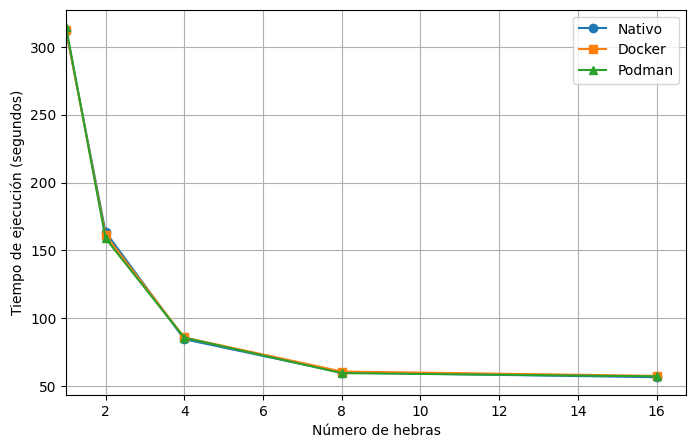
\includegraphics[width=0.8\textwidth]{imagenes/cap5/single-node_ubuntu_container_vs_native_gpu_time.png}
    \caption{Comparativa de tiempo de ejecución entre nativo y contenedores de Ubuntu en función del número de hebras, para CPU + GPU.}
    \label{fig:single-node_ubuntu_container_vs_native_gpu_time}
\end{figure}

En la tabla \ref{tab:single-node_ubuntu_container_vs_native_gpu} se presentan los tiempos de ejecución para ambas configuraciones y la variación porcentual entre ellas.

\begin{table}[ht]
    \centering
    \small
    \setlength{\tabcolsep}{4pt}
    \renewcommand{\arraystretch}{1.1}
    \begin{tabular}{|c|c|c|c|c|c|}
        \hline
        \textbf{Hebras} & \textbf{Nativo (s)} & \textbf{\textit{Docker} (s)} & \textbf{\textit{Docker} $\Delta$\%} & \textbf{\textit{Podman} (s)} & \textbf{\textit{Podman} $\Delta$\%} \\
        \hline
        1.00            & 2515.21             & 2499.09                      & -0.64                               & 2499.16                      & -0.64                               \\
        2.00            & 1253.18             & 1255.95                      & 0.22                                & 1266.51                      & 1.06                                \\
        4.00            & 664.69              & 652.33                       & -1.86                               & 665.38                       & 0.10                                \\
        8.00            & 390.72              & 388.04                       & -0.69                               & 400.51                       & 2.51                                \\
        16.00           & 406.76              & 404.09                       & -0.66                               & 413.53                       & 1.66                                \\
        \hline
    \end{tabular}
    \caption{Comparativa de tiempos de ejecución entre nativo, \textit{Docker} y \textit{Podman} en función del número de hebras y variación porcentual respecto a nativo (CPU + GPU, monoproceso).}
    \label{tab:single-node_ubuntu_container_vs_native_gpu}
\end{table}

La tabla compara los tiempos de ejecución entre los entornos nativo, \textit{Docker} y \textit{Podman} en un escenario monoproceso con CPU + GPU, mostrando también la variación porcentual de los contenedores respecto al entorno nativo para diferentes números de hebras. Los resultados indican que las diferencias de rendimiento entre la ejecución nativa y en contenedores son mínimas. Con una hebra, tanto \textit{Docker} como \textit{Podman} presentan tiempos de ejecución ligeramente inferiores al nativo (reducción del 0.64\%), lo que sugiere que la sobrecarga de los contenedores es prácticamente inexistente en este caso. Al aumentar el número de hebras, las diferencias siguen siendo muy pequeñas: \textit{Docker} oscila entre ligeras mejoras y pequeñas penalizaciones (máximo -1.86\% y 0.22\%), mientras que \textit{Podman} muestra valores similares, con variaciones que no superan el 2.51\%. En conjunto, estos resultados evidencian que el uso de contenedores \textit{Docker} o \textit{Podman} en un entorno monoproceso con CPU + GPU no introduce penalizaciones significativas en el rendimiento respecto a la ejecución nativa, confirmando la viabilidad de ambas tecnologías para la ejecución eficiente de aplicaciones paralelas en este tipo de escenarios.

\subsection{Ejecución en contenedores de Windows}
\subsubsection{CPU}

En la figura \ref{fig:single-node_windows_docker_time} se muestra el tiempo de ejecución para la configuración de CPU en un único proceso con \textit{Docker} en Windows.

\begin{figure}[H]
    \centering
    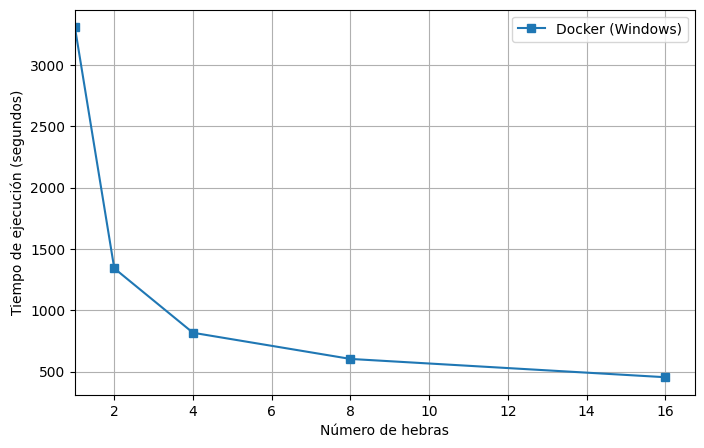
\includegraphics[width=0.8\textwidth]{imagenes/cap5/single-node_windows_docker_time.png}
    \caption{Tiempo de ejecución en un único proceso con \textit{Docker} en Windows (CPU).}
    \label{fig:single-node_windows_docker_time}
\end{figure}

En la tabla \ref{tab:single-node_windows_docker_time} se presentan los tiempos de ejecución y la reducción porcentual respecto a una hebra.

\begin{table}[ht]
    \centering
    \begin{tabular}{|c|c|c|}
        \hline
        \textbf{Hebras} & \textbf{Tiempo (s)} & \textbf{$\Delta$\% vs 1 hebra} \\
        \hline
        1.00            & 3308.08             & 0.00                           \\
        2.00            & 1341.41             & -59.45                         \\
        4.00            & 816.06              & -75.33                         \\
        8.00            & 602.60              & -81.78                         \\
        16.00           & 453.44              & -86.29                         \\
        \hline
    \end{tabular}
    \caption{Tiempos de ejecución y reducción porcentual respecto a una hebra en \textit{Docker} sobre Windows (CPU).}
    \label{tab:single-node_windows_docker_time}
\end{table}

El tiempo de ejecución disminuye de forma significativa al aumentar el número de hebras, alcanzando una reducción del 86.29\% con 16 hebras respecto a la ejecución con una sola hebra.

La mayor mejora relativa se observa al pasar de 1 a 2 hebras (-59.45\%) y de 2 a 4 hebras (-39.46\% adicional), lo que indica una excelente escalabilidad inicial.

A medida que se incrementa el número de hebras, la reducción en el tiempo de ejecución se mantiene, aunque con beneficios marginales decrecientes a partir de 8 hebras.

Estos resultados muestran que, en \textit{Docker} sobre Windows (CPU), el uso de múltiples hebras es muy eficiente y permite aprovechar el paralelismo, siendo recomendable utilizar el mayor número de hebras posible para minimizar el tiempo de ejecución.

En la figura \ref{fig:single-node_windows_podman_time} se muestra el tiempo de ejecución para la configuración de CPU en un único proceso con \textit{Podman} en Windows.

\begin{figure}[H]
    \centering
    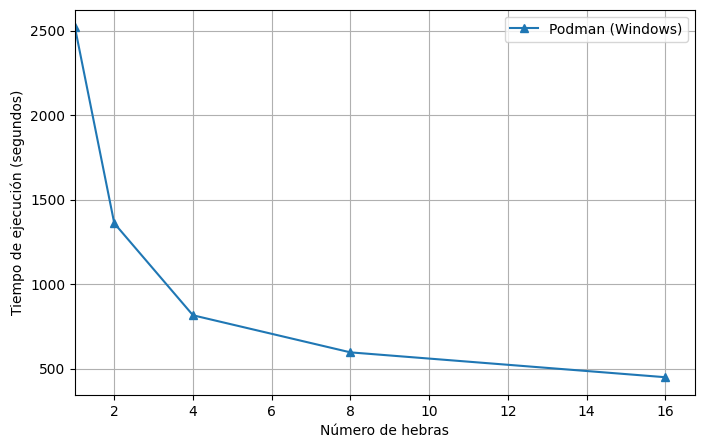
\includegraphics[width=0.8\textwidth]{imagenes/cap5/single-node_windows_podman_time.png}
    \caption{Tiempo de ejecución en un único proceso con \textit{Podman} en Windows (CPU).}
    \label{fig:single-node_windows_podman_time}
\end{figure}

En la tabla \ref{tab:single-node_windows_podman_time} se presentan los tiempos de ejecución y la reducción porcentual respecto a una hebra.

\begin{table}[ht]
    \centering
    \begin{tabular}{|c|c|c|}
        \hline
        \textbf{Hebras} & \textbf{Tiempo (s)} & \textbf{$\Delta$\% vs 1 hebra} \\
        \hline
        1.00            & 2520.21             & 0.00                           \\
        2.00            & 1359.69             & -46.05                         \\
        4.00            & 815.04              & -67.66                         \\
        8.00            & 595.54              & -76.37                         \\
        16.00           & 448.43              & -82.21                         \\
        \hline
    \end{tabular}
    \caption{Tiempos de ejecución y reducción porcentual respecto a una hebra en \textit{Podman} sobre Windows (CPU).}
    \label{tab:single-node_windows_podman_time}
\end{table}

El tiempo de ejecución disminuye notablemente al aumentar el número de hebras, alcanzando una reducción del 82.21\% con 16 hebras respecto a una sola hebra.

La mayor mejora relativa se observa al pasar de 1 a 2 hebras (-46.05\%) y de 2 a 4 hebras (-21.61\% adicional), lo que indica una buena escalabilidad inicial.

A partir de 8 hebras, la reducción en el tiempo de ejecución continúa, aunque los beneficios adicionales son menores, mostrando una tendencia a estabilizarse.

Estos resultados indican que, en \textit{Podman} sobre Windows (CPU), el uso de múltiples hebras es eficiente y permite aprovechar el paralelismo, siendo recomendable utilizar el mayor número de hebras posible para reducir el tiempo de ejecución, aunque las ganancias adicionales disminuyen a partir de 8 hebras.

\subsubsection{CPU + GPU}

% En la figura \ref{fig:single-node_windows_docker_gpu_time} se muestra el tiempo de ejecución para la configuración de CPU + GPU en un único proceso con \textit{Docker} en Windows.

% \begin{figure}[H]
%     \centering
%     \includegraphics[width=0.8\textwidth]{imagenes/cap5/single-node_windows_docker_gpu_time.png}
%     \caption{Tiempo de ejecución en un único proceso con \textit{Docker} en Windows (CPU + GPU).}
%     \label{fig:single-node_windows_docker_gpu_time}
% \end{figure}

% En la tabla \ref{tab:single-node_windows_docker_gpu_time} se presentan los tiempos de ejecución y la reducción porcentual respecto a una hebra.

\subsection{Ejecución en contenedores de Mac}
\subsubsection{CPU}

En la figura \ref{fig:single-node_mac_docker_time} se muestra el tiempo de ejecución para la configuración de CPU en un único proceso con \textit{Docker} en Mac.

\begin{figure}[H]
    \centering
    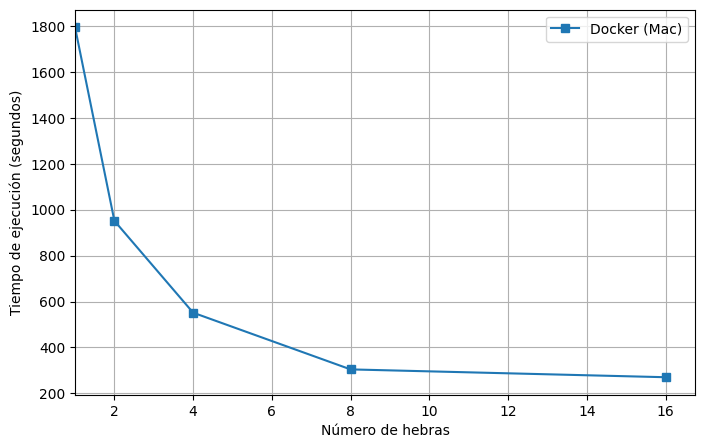
\includegraphics[width=0.8\textwidth]{imagenes/cap5/single-node_mac_docker_time.png}
    \caption{Tiempo de ejecución en un único proceso con \textit{Docker} en Mac (CPU).}
    \label{fig:single-node_mac_docker_time}
\end{figure}

En la tabla \ref{tab:single-node_mac_docker_time} se presentan los tiempos de ejecución y la reducción porcentual respecto a una hebra.

\begin{table}[ht]
    \centering
    \begin{tabular}{|c|c|c|}
        \hline
        \textbf{Hebras} & \textbf{Tiempo (s)} & \textbf{$\Delta$\% vs 1 hebra} \\
        \hline
        1.00            & 1794.98             & 0.00                           \\
        2.00            & 951.56              & -46.99                         \\
        4.00            & 551.41              & -69.28                         \\
        8.00            & 304.35              & -83.04                         \\
        16.00           & 270.25              & -84.94                         \\
        \hline
    \end{tabular}
    \caption{Tiempos de ejecución y reducción porcentual respecto a una hebra en \textit{Docker} sobre Mac (CPU).}
    \label{tab:single-node_mac_docker_time}
\end{table}

El tiempo de ejecución disminuye considerablemente al aumentar el número de hebras, alcanzando una reducción del 84.94\% con 16 hebras respecto a una sola hebra.

La mayor mejora relativa se observa al pasar de 1 a 2 hebras (-46.99\%) y de 2 a 4 hebras (-22.29\% adicional), lo que indica una buena escalabilidad inicial.

A partir de 8 hebras, la reducción en el tiempo de ejecución se estabiliza, con beneficios adicionales menores al incrementar a 16 hebras.

Estos resultados muestran que, en \textit{Docker} sobre Mac (CPU), el uso de múltiples hebras es eficiente y permite aprovechar el paralelismo, siendo recomendable utilizar el mayor número de hebras posible para minimizar el tiempo de ejecución, aunque las ganancias adicionales disminuyen a partir de 8 hebras.

En la figura \ref{fig:single-node_mac_podman_time} se muestra el tiempo de ejecución para la configuración de CPU en un único proceso con \textit{Podman} en Mac.

\begin{figure}[H]
    \centering
    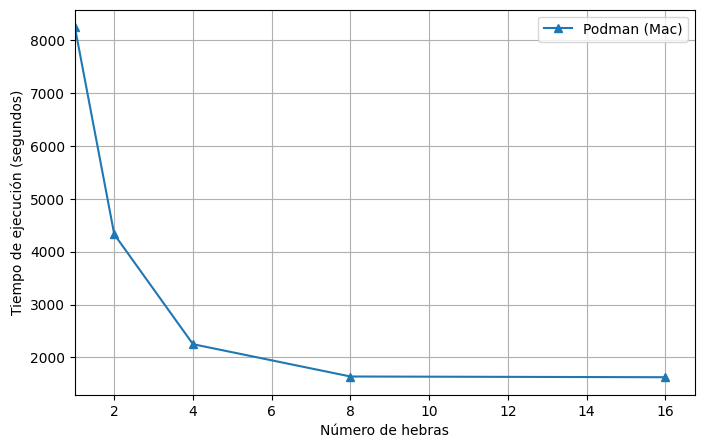
\includegraphics[width=0.8\textwidth]{imagenes/cap5/single-node_mac_podman_time.png}
    \caption{Tiempo de ejecución en un único proceso con \textit{Podman} en Mac (CPU).}
    \label{fig:single-node_mac_podman_time}
\end{figure}

En la tabla \ref{tab:single-node_mac_podman_time} se presentan los tiempos de ejecución y la reducción porcentual respecto a una hebra.

\begin{table}[ht]
    \centering
    \begin{tabular}{|c|c|c|}
        \hline
        \textbf{Hebras} & \textbf{Tiempo (s)} & \textbf{$\Delta$\% vs 1 hebra} \\
        \hline
        1.00            & 8247.00             & 0.00                           \\
        2.00            & 4328.00             & -47.52                         \\
        4.00            & 2250.20             & -72.71                         \\
        8.00            & 1638.79             & -80.13                         \\
        16.00           & 1625.19             & -80.29                         \\
        \hline
    \end{tabular}
    \caption{Tiempos de ejecución y reducción porcentual respecto a una hebra en \textit{Podman} sobre Mac (CPU).}
    \label{tab:single-node_mac_podman_time}
\end{table}

El tiempo de ejecución disminuye de forma muy significativa al aumentar el número de hebras, alcanzando una reducción del 80.29\% con 16 hebras respecto a una sola hebra.

La mayor mejora relativa se observa al pasar de 1 a 2 hebras (-47.52\%) y de 2 a 4 hebras (-25.19\% adicional), lo que indica una buena escalabilidad inicial.

A partir de 8 hebras, la reducción en el tiempo de ejecución se estabiliza, con beneficios adicionales mínimos al incrementar a 16 hebras (solo -0.16\% respecto a 8 hebras).

Estos resultados muestran que, en \textit{Podman} sobre Mac (CPU), el uso de múltiples hebras es eficiente hasta cierto punto, pero las ganancias adicionales más allá de 8 hebras son muy limitadas, sugiriendo que el paralelismo óptimo se alcanza alrededor de ese valor.

\section{Pruebas multiproceso}
\subsection{Ejecución en Ubuntu en nativo}
\subsubsection{CPU}

La figura \ref{fig:multi-node_ubuntu_cpu_native_time} muestra el tiempo de ejecución para la configuración de CPU en un entorno multiproceso con Ubuntu nativo.

\begin{figure}[H]
    \centering
    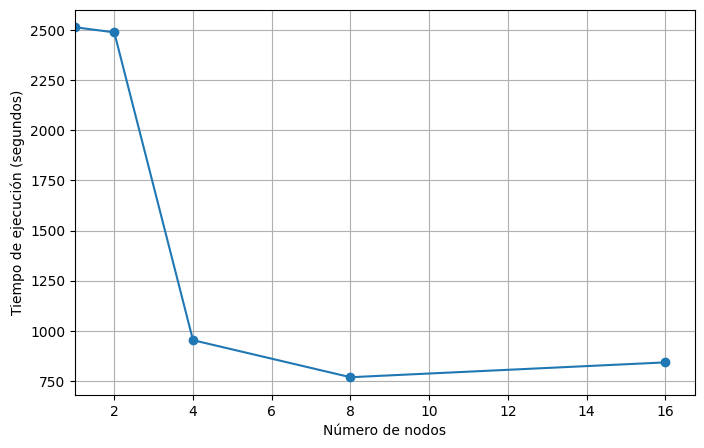
\includegraphics[width=0.8\textwidth]{imagenes/cap5/multi-node_ubuntu_cpu_native_time.png}
    \caption{Tiempo de ejecución en función del número de hebras en Ubuntu nativo (CPU) en entorno multiproceso.}
    \label{fig:multi-node_ubuntu_cpu_native_time}
\end{figure}

En la tabla \ref{tab:multi-node_ubuntu_cpu_native} se presentan los tiempos de ejecución y la variación porcentual respecto a una hebra.

\begin{table}[ht]
    \centering
    \begin{tabular}{|c|c|c|}
        \hline
        \textbf{Procesos} & \textbf{Tiempo de ejecución (s)} & \textbf{$\Delta$\% vs 1 proceso} \\
        \hline
        1                 & 2515.21                          & 0.00                             \\
        2                 & 2489.49                          & -1.02                            \\
        4                 & 952.85                           & -62.12                           \\
        8                 & 767.87                           & -69.47                           \\
        16                & 841.96                           & -66.53                           \\
        \hline
    \end{tabular}
    \caption{Tiempos de ejecución y variación porcentual respecto a un proceso en entorno multiproceso Ubuntu nativo (CPU).}
    \label{tab:multi-node_ubuntu_cpu_native}
\end{table}

La tabla muestra cómo varía el tiempo de ejecución al aumentar el número de procesos en un entorno multiproceso Ubuntu nativo usando CPU. Se observa que:

Al pasar de 1 a 2 procesos, la variación del tiempo es mínima (-1.02\%), lo que indica poca mejora.
Con 4 procesos, el tiempo baja significativamente (-62.12\%), mostrando una mejora notable en la paralelización.
Con 8 procesos, la reducción es aún mayor (69.47\%), aunque el beneficio adicional respecto a 4 procesos es menor.
Al aumentar a 16 procesos, el tiempo de ejecución aumenta ligeramente respecto a 8 procesos y la reducción porcentual disminuye (66.53\%), lo que sugiere que a partir de cierto punto añadir más procesos no mejora el rendimiento e incluso puede empeorarlo, posiblemente por sobrecarga de comunicación o gestión.

En resumen, la eficiencia de la paralelización mejora hasta cierto número de procesos, pero después se observa un efecto de saturación o incluso degradación del rendimiento.

En la figura \ref{fig:multi-node_ubuntu_cpu_native_cpu} se muestra el porcentaje de uso de CPU y la eficiencia en función del número de procesos en un entorno multiproceso con Ubuntu nativo.

\begin{figure}[H]
    \centering
    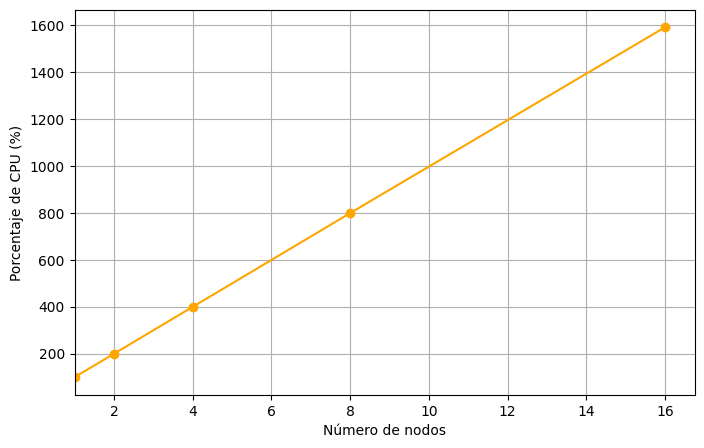
\includegraphics[width=0.8\textwidth]{imagenes/cap5/multi-node_ubuntu_cpu_native_cpu_time.png}
    \caption{Porcentaje de uso de CPU y eficiencia en función del número de procesos en Ubuntu nativo (CPU) en entorno multiproceso.}
    \label{fig:multi-node_ubuntu_cpu_native_cpu}
\end{figure}

En la tabla \ref{tab:multi-node_ubuntu_cpu_native_cpu} se presentan los porcentajes de uso de CPU y la eficiencia correspondiente.

\begin{table}[ht]
    \centering
    \small
    \setlength{\tabcolsep}{4pt}
    \renewcommand{\arraystretch}{1.1}
    \begin{tabular}{|c|c|c|c|}
        \hline
        \textbf{Procesos} & \textbf{Porcentaje de CPU (\%)} & \textbf{Max uso CPU (\%)} & \textbf{Eficiencia CPU (\%)} \\
        \hline
        1                 & 99.00                           & 100.00                    & 99.00                        \\
        2                 & 199.00                          & 200.00                    & 99.50                        \\
        4                 & 399.00                          & 400.00                    & 99.75                        \\
        8                 & 799.00                          & 800.00                    & 99.88                        \\
        16                & 1592.00                         & 1600.00                   & 99.50                        \\
        \hline
    \end{tabular}
    \caption{Porcentaje de uso de CPU y eficiencia en función del número de procesos en Ubuntu nativo (CPU) en entorno multiproceso.}
    \label{tab:multi-node_ubuntu_cpu_native_cpu}
\end{table}

La tabla muestra el porcentaje de uso de CPU y la eficiencia al aumentar el número de procesos en un entorno multiproceso Ubuntu nativo (CPU):

El uso de CPU escala casi linealmente con el número de procesos, lo que indica que los recursos se están utilizando de manera efectiva. El valor "Max uso CPU" representa el uso máximo teórico (número de procesos $\times$ 100\%), y el uso real está muy cerca de ese máximo en todos los casos. La eficiencia de CPU se mantiene muy alta (entre 99.00\% y 99.88\%) para todos los escenarios, lo que sugiere que la sobrecarga de paralelización es mínima y que el sistema aprovecha casi todo el potencial de los recursos disponibles. Solo con 16 procesos se observa una ligera caída en la eficiencia (99.50\%), pero sigue siendo excelente.

En resumen, el sistema mantiene una eficiencia de CPU muy alta al escalar el número de procesos, lo que indica una buena gestión de los recursos y una paralelización efectiva en este entorno.

\subsubsection{CPU + GPU}

La figura \ref{fig:multi-node_ubuntu_gpu_native_time} muestra el tiempo de ejecución para la configuración de CPU + GPU en un entorno multiproceso con Ubuntu nativo.

\begin{figure}[H]
    \centering
    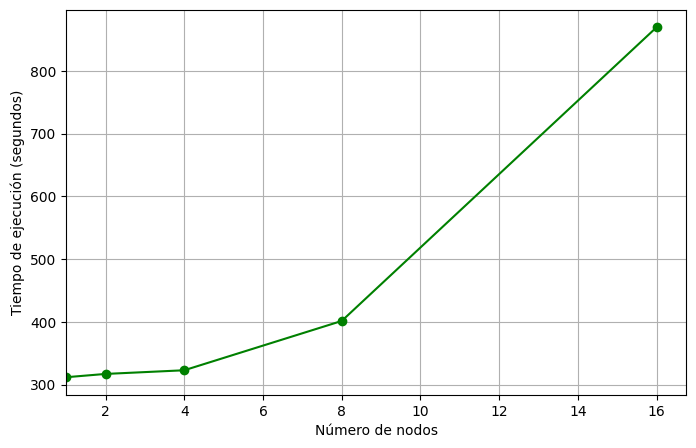
\includegraphics[width=0.8\textwidth]{imagenes/cap5/multi-node_ubuntu_gpu_native_time.png}
    \caption{Tiempo de ejecución en función del número de hebras en Ubuntu nativo (CPU + GPU) en entorno multiproceso.}
    \label{fig:multi-node_ubuntu_gpu_native_time}
\end{figure}

En la tabla \ref{tab:multi-node_ubuntu_gpu_native} se presentan los tiempos de ejecución y la variación porcentual respecto a una hebra.

\begin{table}[ht]
    \centering
    \begin{tabular}{|c|c|c|}
        \hline
        \textbf{Procesos} & \textbf{Tiempo (s)} & \textbf{$\Delta$\% vs 1 proceso} \\
        \hline
        1                 & 311.68              & 0.00                             \\
        2                 & 316.92              & 1.68                             \\
        4                 & 322.77              & 3.56                             \\
        8                 & 401.33              & 28.76                            \\
        16                & 869.40              & 178.94                           \\
        \hline
    \end{tabular}
    \caption{Tiempos de ejecución y variación porcentual respecto a un proceso en entorno multiproceso Ubuntu nativo (CPU + GPU).}
    \label{tab:multi-node_ubuntu_gpu_native}
\end{table}

La tabla muestra los tiempos de ejecución y la variación porcentual al aumentar el número de procesos en un entorno multiproceso Ubuntu nativo utilizando CPU y GPU:

Con un solo proceso, el tiempo base es de 311.68\,s. Al incrementar a 2 y 4 procesos, el tiempo de ejecución aumenta ligeramente (316.92\,s y 322.77\,s), lo que implica una pequeña penalización en lugar de una mejora (variaciones positivas del 1.68\% y 3.56\%). Con 8 procesos, el tiempo sube notablemente hasta 401.33\,s (+28.76\%), y con 16 procesos el incremento es aún mayor (869.40\,s, +178.94\%).

Estos resultados indican que, a diferencia del caso solo CPU, al añadir más procesos con GPU el rendimiento empeora progresivamente. Es probable que la sobrecarga de comunicación, la gestión de recursos compartidos o la falta de escalabilidad de la aplicación para GPU estén afectando negativamente. En este entorno, la paralelización no solo no aporta beneficios, sino que resulta contraproducente a partir de más de un proceso.

\subsubsection{Comparativa CPU vs CPU + GPU}

En la figura \ref{fig:multi-node_ubuntu_cpu_vs_gpu_native_time} se muestra una comparativa del tiempo de ejecución entre las configuraciones CPU y CPU + GPU en un entorno multiproceso con Ubuntu nativo.

\begin{figure}[H]
    \centering
    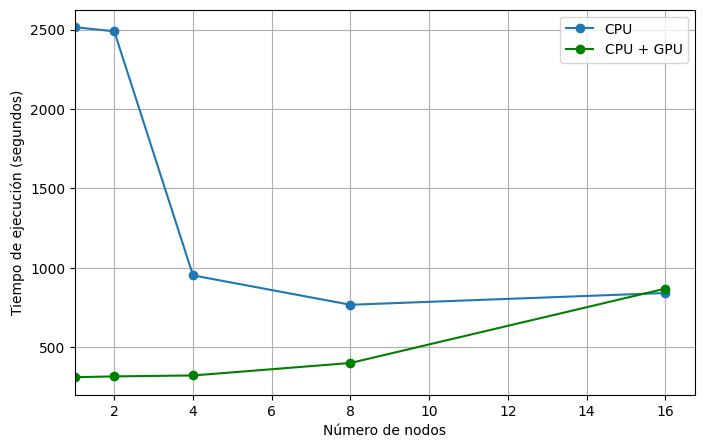
\includegraphics[width=0.8\textwidth]{imagenes/cap5/multi-node_ubuntu_cpu_vs_gpu_native_time.png}
    \caption{Comparativa de tiempo de ejecución entre CPU y CPU + GPU en función del número de procesos en Ubuntu nativo en entorno multiproceso.}
    \label{fig:multi-node_ubuntu_cpu_vs_gpu_native_time}
\end{figure}

En la tabla \ref{tab:multi-node_ubuntu_cpu_vs_gpu_native} se presentan los tiempos de ejecución para ambas configuraciones y la variación porcentual entre ellas.

\begin{table}[ht]
    \centering
    \begin{tabular}{|c|c|c|c|}
        \hline
        \textbf{Procesos} & \textbf{Tiempo CPU (s)} & \textbf{Tiempo CPU+GPU (s)} & \textbf{Variación (\%)} \\
        \hline
        1                 & 2515.21                 & 311.68                      & -87.61                  \\
        2                 & 2489.49                 & 316.92                      & -87.27                  \\
        4                 & 952.85                  & 322.77                      & -66.13                  \\
        8                 & 767.87                  & 401.33                      & -47.73                  \\
        16                & 841.96                  & 869.40                      & 3.26                    \\
        \hline
    \end{tabular}
    \caption{Comparativa de tiempos de ejecución entre CPU y CPU+GPU en función del número de procesos en Ubuntu nativo (multiproceso) y variación porcentual.}
    \label{tab:multi-node_ubuntu_cpu_vs_gpu_native}
\end{table}

La tabla muestra que, con uno y dos procesos, la configuración CPU+GPU es considerablemente más rápida que la opción solo CPU, con reducciones de tiempo superiores al 87\%. Esto evidencia un beneficio claro del uso de GPU en escenarios con pocos procesos. Al aumentar a cuatro y ocho procesos, la ventaja de la GPU disminuye: la reducción es del 66.13\% con cuatro procesos y del 47.73\% con ocho procesos. Aunque la GPU sigue proporcionando mejores tiempos, la diferencia se reduce conforme se incrementa el número de procesos. Con dieciséis procesos, la situación se invierte y el tiempo de CPU+GPU resulta ligeramente superior al de solo CPU, con una variación positiva del 3.26\%. Esto sugiere que, a partir de cierto punto, la sobrecarga asociada al uso de GPU y la comunicación entre procesos supera los beneficios de la aceleración.

En resumen, el uso de GPU aporta grandes mejoras en los tiempos de ejecución para un bajo número de procesos, pero su escalabilidad es limitada. A medida que se incrementa el número de procesos, la eficiencia de la GPU disminuye y puede llegar a ser contraproducente, probablemente debido a la sobrecarga de comunicación y la gestión de recursos en entornos multiproceso.

\subsection{Ejecución en contenedores de Ubuntu}
\subsubsection{CPU}

En la figura \ref{fig:multi-node_ubuntu_docker_time} se muestra el tiempo de ejecución para la configuración de CPU en un entorno multiproceso con contenedores de Ubuntu.

\begin{figure}[H]
    \centering
    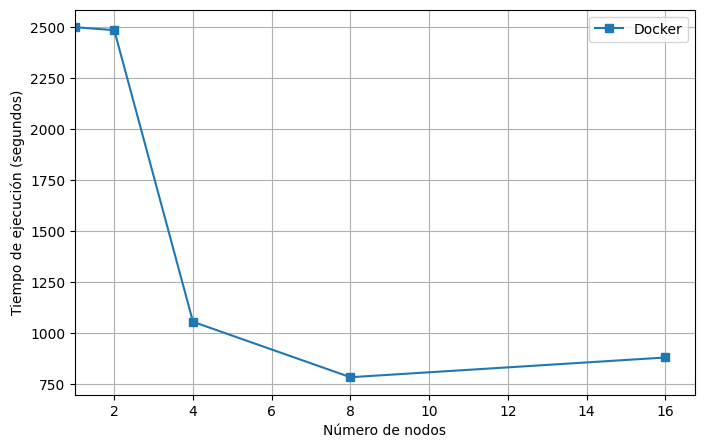
\includegraphics[width=0.8\textwidth]{imagenes/cap5/multi-node_ubuntu_docker_time.png}
    \caption{Tiempo de ejecución en función del número de hebras en contenedores de Ubuntu (CPU) en entorno multiproceso.}
    \label{fig:multi-node_ubuntu_docker_time}
\end{figure}

En la tabla \ref{tab:multi-node_ubuntu_docker} se presentan los tiempos de ejecución y la variación porcentual respecto a una hebra.

\begin{table}[ht]
    \centering
    \begin{tabular}{|c|c|c|}
        \hline
        \textbf{Procesos} & \textbf{Tiempo (s)} & \textbf{$\Delta$\% vs 1 proceso} \\
        \hline
        1                 & 2499.09             & 0.00                             \\
        2                 & 2484.80             & -0.57                            \\
        4                 & 1054.20             & -57.82                           \\
        8                 & 782.42              & -68.69                           \\
        16                & 879.20              & -64.82                           \\
        \hline
    \end{tabular}
    \caption{Tiempos de ejecución y variación porcentual respecto a un proceso en entorno multiproceso con contenedores de Ubuntu (CPU).}
    \label{tab:multi-node_ubuntu_docker}
\end{table}

De 1 a 2 procesos, la mejora es mínima (-0.57\%), lo que indica que la paralelización apenas aporta beneficio en este rango. Con 4 procesos, la reducción es significativa (57.82\%), mostrando una mejora clara en el rendimiento gracias a la paralelización. Con 8 procesos, la reducción alcanza el 68.69\%, lo que indica un buen aprovechamiento de los recursos al escalar. Con 16 procesos, el tiempo de ejecución aumenta ligeramente respecto a 8 procesos y la reducción porcentual disminuye a -64.82\%, lo que sugiere que a partir de cierto punto la eficiencia se ve limitada, posiblemente por la sobrecarga de coordinación y comunicación entre contenedores.

En resumen, el entorno con contenedores de Ubuntu permite una buena escalabilidad hasta 8 procesos, con mejoras notables en el tiempo de ejecución. Sin embargo, al aumentar a 16 procesos, la eficiencia disminuye, mostrando un comportamiento similar al entorno nativo: la paralelización es efectiva hasta cierto límite, tras el cual la sobrecarga afecta negativamente al rendimiento.

En la figura \ref{fig:multi-node_ubuntu_podman} se muestra el tiempo de ejecución para la configuración de CPU en un entorno multiproceso con contenedores de \textit{Podman}.

\begin{figure}[H]
    \centering
    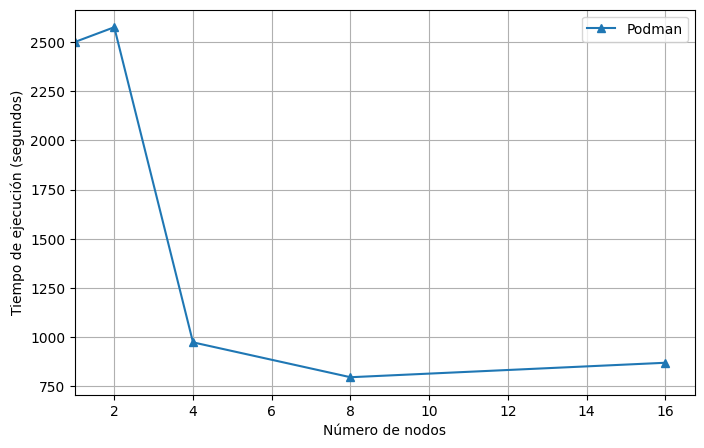
\includegraphics[width=0.8\textwidth]{imagenes/cap5/multi-node_ubuntu_podman_time.png}
    \caption{Tiempo de ejecución en función del número de hebras en contenedores de \textit{Podman} (CPU) en entorno multiproceso.}
    \label{fig:multi-node_ubuntu_podman}
\end{figure}

En la tabla \ref{tab:multi-node_ubuntu_podman} se presentan los tiempos de ejecución y la reducción porcentual respecto a una hebra.

\begin{table}[ht]
    \centering
    \begin{tabular}{|c|c|c|}
        \hline
        \textbf{Procesos} & \textbf{Tiempo (s)} & \textbf{$\Delta$\% vs 1 proceso} \\
        \hline
        1                 & 2499.16             & 0.00                             \\
        2                 & 2574.04             & 3.00                             \\
        4                 & 973.92              & -61.03                           \\
        8                 & 796.84              & -68.12                           \\
        16                & 870.28              & -65.18                           \\
        \hline
    \end{tabular}
    \caption{Tiempos de ejecución y reducción porcentual respecto a un proceso en entorno multiproceso con contenedores de \textit{Podman} (CPU).}
    \label{tab:multi-node_ubuntu_podman}
\end{table}

La tabla muestra cómo varía el tiempo de ejecución al aumentar el número de procesos en un entorno multiproceso utilizando contenedores de \textit{Podman} sobre CPU. Con un solo proceso se establece el tiempo base, mientras que al duplicar el número de procesos a dos, se observa un ligero aumento en el tiempo de ejecución, lo que indica que la paralelización no solo no aporta mejoras en este caso, sino que introduce una pequeña penalización, probablemente debida a la sobrecarga de gestión de los contenedores. Sin embargo, al incrementar a cuatro procesos, el tiempo de ejecución disminuye considerablemente, reflejando una reducción del 61.03\% respecto al caso de un proceso, lo que evidencia una mejora significativa en el rendimiento gracias a la paralelización. Esta tendencia positiva se mantiene con ocho procesos, donde la reducción alcanza el 68.12\%, mostrando un buen aprovechamiento de los recursos disponibles. No obstante, al aumentar a dieciséis procesos, el tiempo de ejecución vuelve a incrementarse ligeramente y la reducción porcentual disminuye a 65.18\%, lo que sugiere que, a partir de cierto punto, la eficiencia de la paralelización se ve limitada, posiblemente por la sobrecarga de coordinación y comunicación entre los contenedores. En conjunto, el entorno con \textit{Podman} permite una escalabilidad efectiva hasta un número intermedio de procesos, pero muestra limitaciones cuando se incrementa excesivamente el grado de paralelismo.

\subsubsection{CPU + GPU}

En la figura \ref{fig:multi-node_ubuntu_docker_gpu_time} se muestra el tiempo de ejecución para la configuración de CPU + GPU en un entorno multiproceso con contenedores de Ubuntu.

\begin{figure}[H]
    \centering
    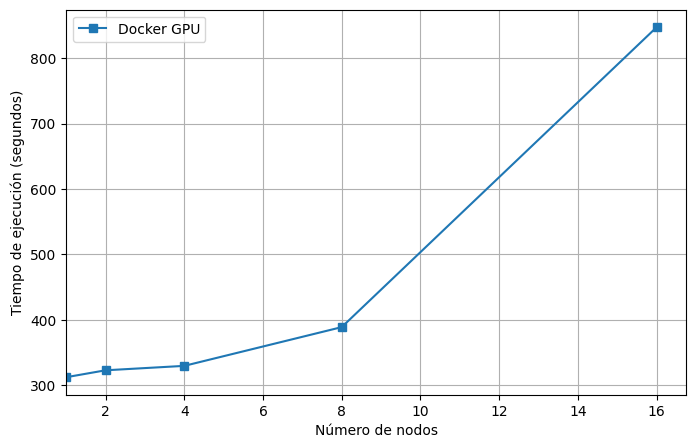
\includegraphics[width=0.8\textwidth]{imagenes/cap5/multi-node_ubuntu_docker_gpu_time.png}
    \caption{Tiempo de ejecución en función del número de hebras en contenedores de Ubuntu (CPU + GPU) en entorno multiproceso.}
    \label{fig:multi-node_ubuntu_docker_gpu_time}
\end{figure}

En la tabla \ref{tab:multi-node_ubuntu_docker_gpu} se presentan los tiempos de ejecución y la reducción porcentual respecto a una hebra.

\begin{table}[ht]
    \centering
    \begin{tabular}{|c|c|c|}
        \hline
        \textbf{Procesos} & \textbf{Tiempo (s)} & \textbf{$\Delta$\% vs 1 proceso} \\
        \hline
        1                 & 312.18              & 0.00                             \\
        2                 & 322.77              & 3.39                             \\
        4                 & 329.54              & 5.56                             \\
        8                 & 388.78              & 24.54                            \\
        16                & 847.37              & 171.44                           \\
        \hline
    \end{tabular}
    \caption{Tiempos de ejecución y variación porcentual respecto a un proceso en entorno multiproceso con contenedores de Ubuntu (CPU + GPU).}
    \label{tab:multi-node_ubuntu_docker_gpu}
\end{table}

La tabla refleja el comportamiento del tiempo de ejecución al aumentar el número de procesos en un entorno multiproceso con contenedores de Ubuntu utilizando tanto CPU como GPU. Con un solo proceso, el tiempo de ejecución es el más bajo, sirviendo como referencia para el resto de configuraciones. Al incrementar a dos y cuatro procesos, lejos de mejorar, el tiempo de ejecución aumenta ligeramente, lo que se traduce en una variación porcentual positiva y evidencia que la paralelización en este contexto no resulta beneficiosa, probablemente debido a la sobrecarga de coordinación y a la gestión de recursos entre los contenedores y las GPUs. Esta tendencia se acentúa al llegar a ocho procesos, donde el tiempo de ejecución sigue incrementándose y la penalización alcanza el 24.54\%. Finalmente, con dieciséis procesos, el tiempo de ejecución se eleva de forma considerable, con una variación porcentual del 171.44\% respecto al caso de un solo proceso. Estos resultados indican que, en este entorno, la escalabilidad es muy limitada y que el uso combinado de contenedores y GPU no solo no aporta mejoras al aumentar el número de procesos, sino que puede llegar a ser claramente contraproducente, probablemente por la complejidad añadida en la gestión de los recursos y la comunicación entre procesos.

En la figura \ref{fig:multi-node_ubuntu_podman_gpu_time} se muestra el tiempo de ejecución para la configuración de CPU + GPU en un entorno multiproceso con contenedores de \textit{Podman}.

\begin{figure}[H]
    \centering
    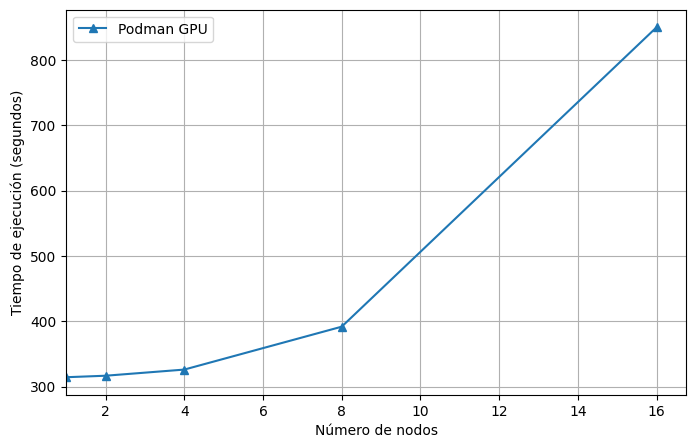
\includegraphics[width=0.8\textwidth]{imagenes/cap5/multi-node_ubuntu_podman_gpu_time.png}
    \caption{Tiempo de ejecución en función del número de hebras en contenedores de \textit{Podman} (CPU + GPU) en entorno multiproceso.}
    \label{fig:multi-node_ubuntu_podman_gpu_time}
\end{figure}

En la tabla \ref{tab:multi-node_ubuntu_podman_gpu} se presentan los tiempos de ejecución y la reducción porcentual respecto a una hebra.

\begin{table}[ht]
    \centering
    \begin{tabular}{|c|c|c|}
        \hline
        \textbf{Procesos} & \textbf{Tiempo (s)} & \textbf{$\Delta$\% vs 1 proceso} \\
        \hline
        1                 & 314.51              & 0.00                             \\
        2                 & 316.80              & 0.73                             \\
        4                 & 326.20              & 3.72                             \\
        8                 & 391.86              & 24.59                            \\
        16                & 850.18              & 170.32                           \\
        \hline
    \end{tabular}
    \caption{Tiempos de ejecución y variación porcentual respecto a un proceso en entorno multiproceso con contenedores de \textit{Podman} (CPU + GPU).}
    \label{tab:multi-node_ubuntu_podman_gpu}
\end{table}

La tabla muestra la evolución del tiempo de ejecución al aumentar el número de procesos en un entorno multiproceso con contenedores de \textit{Podman} utilizando tanto CPU como GPU. Con un solo proceso, el tiempo de ejecución es el más bajo y sirve como referencia. Al pasar a dos y cuatro procesos, se observa un ligero incremento en el tiempo de ejecución, con variaciones porcentuales positivas que indican que la paralelización no aporta mejoras y, de hecho, introduce una pequeña penalización, probablemente debida a la sobrecarga de coordinación y gestión de recursos entre los contenedores y las GPUs. Esta tendencia se intensifica al aumentar a ocho procesos, donde el tiempo de ejecución crece de manera más notable y la penalización alcanza el 24.59\%. Finalmente, con dieciséis procesos, el tiempo de ejecución se incrementa considerablemente, con una variación porcentual del 170.32\% respecto al caso de un solo proceso. Estos resultados evidencian que, en este entorno, la escalabilidad es muy limitada y que el uso combinado de contenedores \textit{Podman} y GPU no solo no mejora el rendimiento al aumentar el número de procesos, sino que puede resultar claramente perjudicial, probablemente debido a la complejidad añadida en la gestión de recursos y la comunicación entre procesos.

\subsubsection{Comparativa contenedores vs nativo}

En la figura \ref{fig:multi-node_ubuntu_container_vs_native_time} se muestra una comparativa del tiempo de ejecución entre las configuraciones nativo y contenedores de Ubuntu en un entorno multiproceso con CPU.

\begin{figure}[H]
    \centering
    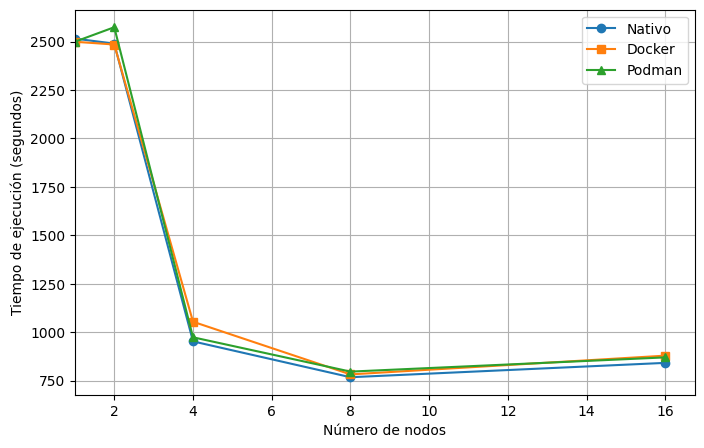
\includegraphics[width=0.8\textwidth]{imagenes/cap5/multi-node_ubuntu_container_vs_native_time.png}
    \caption{Comparativa de tiempo de ejecución entre nativo y contenedores de Ubuntu en función del número de procesos en entorno multiproceso (CPU).}
    \label{fig:multi-node_ubuntu_container_vs_native_time}
\end{figure}

En la tabla \ref{tab:multi-node_ubuntu_container_vs_native} se presentan los tiempos de ejecución para ambas configuraciones y la variación porcentual entre ellas.

\begin{table}[ht]
    \centering
    \small
    \setlength{\tabcolsep}{4pt}
    \renewcommand{\arraystretch}{1.1}
    \begin{tabular}{|c|c|c|c|c|c|}
        \hline
        \textbf{Procesos} & \textbf{Nativo (s)} & \textbf{\textit{Docker} (s)} & \textbf{\textit{Docker} $\Delta$\%} & \textbf{\textit{Podman} (s)} & \textbf{\textit{Podman} $\Delta$\%} \\
        \hline
        1                 & 2515.21             & 2499.09                      & -0.64                               & 2499.16                      & -0.64                               \\
        2                 & 2489.49             & 2484.80                      & -0.19                               & 2574.04                      & 3.40                                \\
        4                 & 952.85              & 1054.20                      & 10.64                               & 973.92                       & 2.21                                \\
        8                 & 767.87              & 782.42                       & 1.89                                & 796.84                       & 3.77                                \\
        16                & 841.96              & 879.20                       & 4.42                                & 870.28                       & 3.36                                \\
        \hline
    \end{tabular}
    \caption{Comparativa de tiempos de ejecución entre nativo, \textit{Docker} y \textit{Podman} en función del número de procesos en entorno multiproceso (CPU) y variación porcentual respecto a nativo.}
    \label{tab:multi-node_ubuntu_container_vs_native}
\end{table}

La tabla presenta una comparación de los tiempos de ejecución entre los entornos nativo, \textit{Docker} y \textit{Podman} en un escenario multiproceso utilizando únicamente CPU, así como la variación porcentual de los contenedores respecto al entorno nativo. Con un solo proceso, tanto \textit{Docker} como \textit{Podman} muestran tiempos de ejecución ligeramente inferiores al nativo, con una reducción del 0.64\%, lo que indica que la sobrecarga de los contenedores es prácticamente inexistente en este caso. Al aumentar a dos procesos, \textit{Docker} mantiene una ligera mejora, mientras que \textit{Podman} experimenta un incremento del 3.40\% en el tiempo de ejecución, sugiriendo que la eficiencia de los contenedores puede variar según la tecnología empleada y la carga de trabajo. Con cuatro procesos, \textit{Docker} presenta un aumento notable del 10.64\% respecto al nativo, mientras que \textit{Podman} solo incrementa un 2.21\%, lo que podría estar relacionado con la gestión interna de los recursos y la coordinación entre contenedores. A medida que se incrementa el número de procesos a ocho y dieciséis, tanto \textit{Docker} como \textit{Podman} muestran incrementos moderados en los tiempos de ejecución respecto al entorno nativo, aunque las diferencias se mantienen en valores relativamente bajos. En conjunto, los resultados indican que el uso de contenedores en entornos multiproceso con CPU introduce una sobrecarga mínima o moderada en la mayoría de los casos, siendo \textit{Docker} algo más sensible a la escalabilidad en configuraciones intermedias. Sin embargo, la viabilidad de los contenedores para la ejecución de aplicaciones paralelas y distribuidas se mantiene, ya que las diferencias de rendimiento respecto al entorno nativo no son excesivamente significativas.

En la figura \ref{fig:multi-node_ubuntu_container_vs_native_gpu_time} se muestra una comparativa del tiempo de ejecución entre las configuraciones nativo y contenedores de Ubuntu en un entorno multiproceso con CPU + GPU.

\begin{figure}[H]
    \centering
    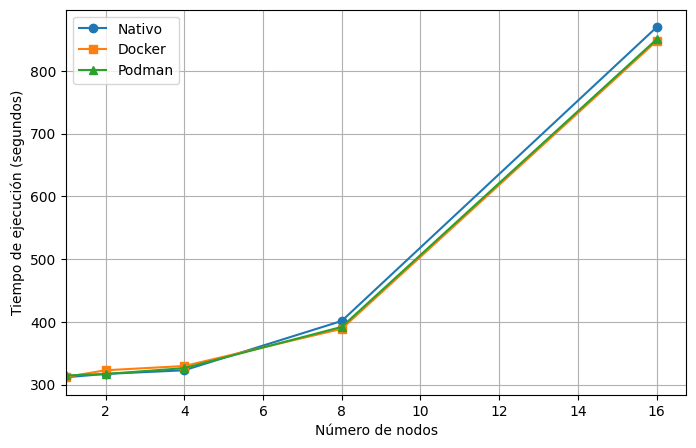
\includegraphics[width=0.8\textwidth]{imagenes/cap5/multi-node_ubuntu_container_vs_native_gpu_time.png}
    \caption{Comparativa de tiempo de ejecución entre nativo y contenedores de Ubuntu en función del número de procesos en entorno multiproceso (CPU + GPU).}
    \label{fig:multi-node_ubuntu_container_vs_native_gpu_time}
\end{figure}

En la tabla \ref{tab:multi-node_ubuntu_container_vs_native_gpu} se presentan los tiempos de ejecución para ambas configuraciones y la variación porcentual entre ellas.

\begin{table}[ht]
    \centering
    \small
    \setlength{\tabcolsep}{4pt}
    \renewcommand{\arraystretch}{1.1}
    \begin{tabular}{|c|c|c|c|c|c|}
        \hline
        \textbf{Procesos} & \textbf{Nativo (s)} & \textbf{\textit{Docker} (s)} & \textbf{\textit{Docker} $\Delta$\%} & \textbf{\textit{Podman} (s)} & \textbf{\textit{Podman} $\Delta$\%} \\
        \hline
        1                 & 311.68              & 312.18                       & 0.16                                & 314.51                       & 0.91                                \\
        2                 & 316.92              & 322.77                       & 1.85                                & 316.80                       & -0.04                               \\
        4                 & 322.77              & 329.54                       & 2.10                                & 326.20                       & 1.06                                \\
        8                 & 401.33              & 388.78                       & -3.13                               & 391.86                       & -2.36                               \\
        16                & 869.40              & 847.37                       & -2.53                               & 850.18                       & -2.21                               \\
        \hline
    \end{tabular}
    \caption{Comparativa de tiempos de ejecución entre nativo, \textit{Docker} y \textit{Podman} en función del número de procesos en entorno multiproceso (CPU+GPU) y variación porcentual respecto a nativo.}
    \label{tab:multi-node_ubuntu_container_vs_native_gpu}
\end{table}

La tabla compara los tiempos de ejecución en un entorno multiproceso con CPU y GPU para las configuraciones nativa, \textit{Docker} y \textit{Podman}, mostrando también la variación porcentual de los contenedores respecto al entorno nativo. Con un solo proceso, tanto \textit{Docker} como \textit{Podman} presentan tiempos de ejecución prácticamente idénticos al entorno nativo, con diferencias inferiores al 1\%, lo que indica que la sobrecarga de los contenedores es despreciable en este escenario. Al aumentar a dos y cuatro procesos, \textit{Docker} muestra un ligero incremento en el tiempo de ejecución respecto al nativo, mientras que \textit{Podman} se mantiene prácticamente igual o con una diferencia muy pequeña, lo que sugiere que ambos sistemas de contenedores gestionan eficientemente la paralelización en estos casos. Sin embargo, al escalar a ocho y dieciséis procesos, tanto \textit{Docker} como \textit{Podman} presentan tiempos de ejecución ligeramente inferiores a los del entorno nativo, con variaciones negativas que indican una mejora marginal en el rendimiento. Este comportamiento puede deberse a pequeñas diferencias en la gestión de recursos o a la forma en que los contenedores distribuyen la carga de trabajo. En conjunto, los resultados muestran que el uso de contenedores, tanto \textit{Docker} como \textit{Podman}, no introduce penalizaciones significativas en el rendimiento respecto al entorno nativo y, en algunos casos, incluso puede aportar ligeras mejoras al aumentar el número de procesos, lo que demuestra la viabilidad de estas tecnologías para la ejecución de aplicaciones paralelas y distribuidas en entornos multiproceso con aceleración por GPU.

\subsection{Ejecución en contenedores de Windows}
\subsubsection{CPU}

En la figura \ref{fig:multi-node_windows_docker_time} se muestra el tiempo de ejecución para la configuración de CPU en un entorno multiproceso con contenedores de Windows.

\begin{figure}[H]
    \centering
    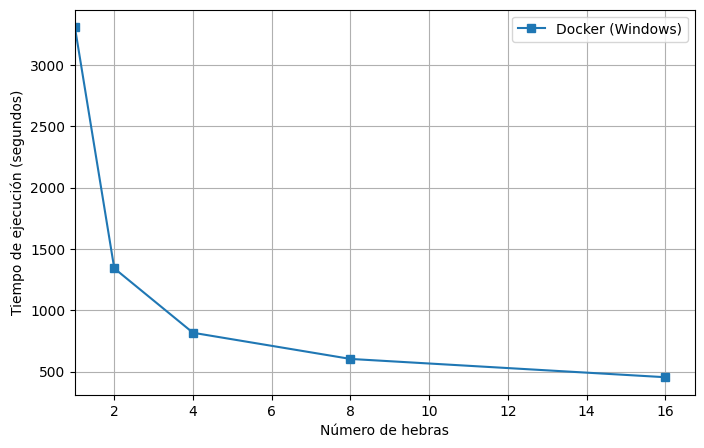
\includegraphics[width=0.8\textwidth]{imagenes/cap5/multi-node_windows_docker_time.png}
    \caption{Tiempo de ejecución en función del número de hebras en contenedores de Windows (CPU) en entorno multiproceso.}
    \label{fig:multi-node_windows_docker_time}
\end{figure}

En la tabla \ref{tab:multi-node_windows_docker} se presentan los tiempos de ejecución y la reducción porcentual respecto a una hebra.

\begin{table}[ht]
    \centering
    \begin{tabular}{|c|c|c|}
        \hline
        \textbf{Procesos} & \textbf{Tiempo (s)} & \textbf{$\Delta$\% vs 1 proceso} \\
        \hline
        1                 & 3308.08             & 0.00                             \\
        2                 & 2708.91             & -18.11                           \\
        4                 & 1185.46             & -64.16                           \\
        8                 & 1090.62             & -67.03                           \\
        16                & 930.79              & -71.86                           \\
        \hline
    \end{tabular}
    \caption{Tiempos de ejecución y reducción porcentual respecto a un proceso en entorno multiproceso con contenedores de Windows (CPU).}
    \label{tab:multi-node_windows_docker}
\end{table}

La tabla muestra la evolución del tiempo de ejecución al aumentar el número de procesos en un entorno multiproceso con contenedores de Windows utilizando CPU. Con un solo proceso, el tiempo de ejecución es el más alto y sirve como referencia para el resto de configuraciones. Al duplicar el número de procesos a dos, se observa una reducción significativa del 18.11\% en el tiempo de ejecución, lo que indica que la paralelización comienza a aportar beneficios claros. Esta mejora se acentúa al incrementar a cuatro procesos, donde la reducción alcanza el 64.16\%, reflejando una eficiencia notable en la distribución de la carga de trabajo. Con ocho procesos, la reducción porcentual es del 67.03\%, lo que demuestra que el sistema sigue escalando de manera eficiente. Finalmente, al llegar a dieciséis procesos, el tiempo de ejecución disminuye aún más, con una reducción del 71.86\% respecto al caso de un solo proceso. Estos resultados evidencian que el entorno multiproceso con contenedores de Windows permite una escalabilidad efectiva y un aprovechamiento eficiente de los recursos al aumentar el número de procesos, logrando mejoras sustanciales en el rendimiento conforme se incrementa el grado de paralelismo.

En la figura \ref{fig:multi-node_windows_podman_time} se muestra el tiempo de ejecución para la configuración de CPU en un entorno multiproceso con contenedores de \textit{Podman} en Windows.

\begin{figure}[H]
    \centering
    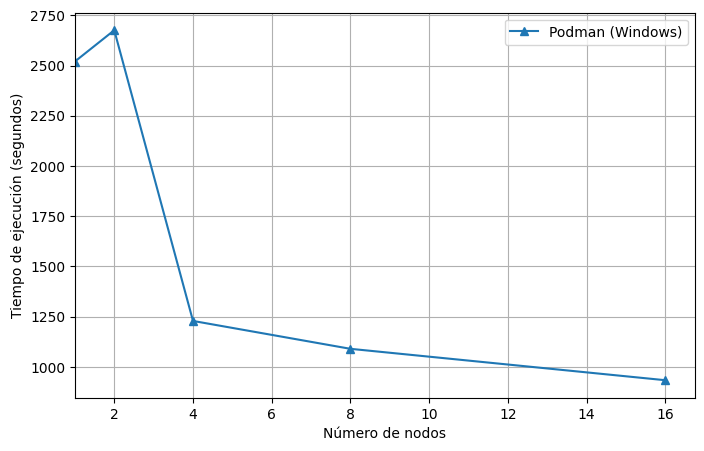
\includegraphics[width=0.8\textwidth]{imagenes/cap5/multi-node_windows_podman_time.png}
    \caption{Tiempo de ejecución en función del número de hebras en contenedores de \textit{Podman} (CPU) en entorno multiproceso.}
    \label{fig:multi-node_windows_podman_time}
\end{figure}

En la tabla \ref{tab:multi-node_windows_podman} se presentan los tiempos de ejecución y la reducción porcentual respecto a una hebra.

\begin{table}[ht]
    \centering
    \begin{tabular}{|c|c|c|}
        \hline
        \textbf{Procesos} & \textbf{Tiempo (s)} & \textbf{$\Delta$\% vs 1 proceso} \\
        \hline
        1.00              & 2520.21             & 0.00                             \\
        2.00              & 2675.94             & 6.18                             \\
        4.00              & 1228.59             & -51.25                           \\
        8.00              & 1089.75             & -56.76                           \\
        16.00             & 933.45              & -62.96                           \\
        \hline
    \end{tabular}
    \caption{Tiempos de ejecución y reducción porcentual respecto a un proceso en entorno multiproceso con contenedores de \textit{Podman} en Windows (CPU).}
    \label{tab:multi-node_windows_podman}
\end{table}

La tabla presenta la evolución del tiempo de ejecución al aumentar el número de procesos en un entorno multiproceso con contenedores de \textit{Podman} sobre Windows utilizando CPU. Con un solo proceso, se establece el tiempo de referencia. Al pasar a dos procesos, se observa un incremento del 6.18\% en el tiempo de ejecución, lo que indica que la paralelización en este caso introduce una penalización inicial, probablemente debida a la sobrecarga de coordinación o a la gestión de recursos en el entorno de contenedores sobre Windows. Sin embargo, al aumentar a cuatro procesos, el tiempo de ejecución disminuye de forma considerable, con una reducción del 51.25\%, lo que evidencia una mejora significativa en el rendimiento gracias a la paralelización. Esta tendencia positiva se mantiene al escalar a ocho y dieciséis procesos, donde las reducciones alcanzan el 56.76\% y el 62.96\% respectivamente, mostrando que el sistema es capaz de aprovechar de manera eficiente los recursos adicionales a medida que se incrementa el número de procesos. En conjunto, los resultados indican que, aunque existe una penalización inicial al duplicar los procesos, el entorno multiproceso con contenedores de \textit{Podman} en Windows logra una escalabilidad efectiva y una mejora sustancial del rendimiento a partir de cuatro procesos, confirmando la viabilidad de esta tecnología para la ejecución de aplicaciones paralelas en este contexto.

\subsubsection{CPU + GPU}

\subsection{Ejecución en contenedores de Mac}
\subsubsection{CPU}

En la figura \ref{fig:multi-node_mac_docker_time} se muestra el tiempo de ejecución para la configuración de CPU en un entorno multiproceso con contenedores de Mac.

\begin{figure}[H]
    \centering
    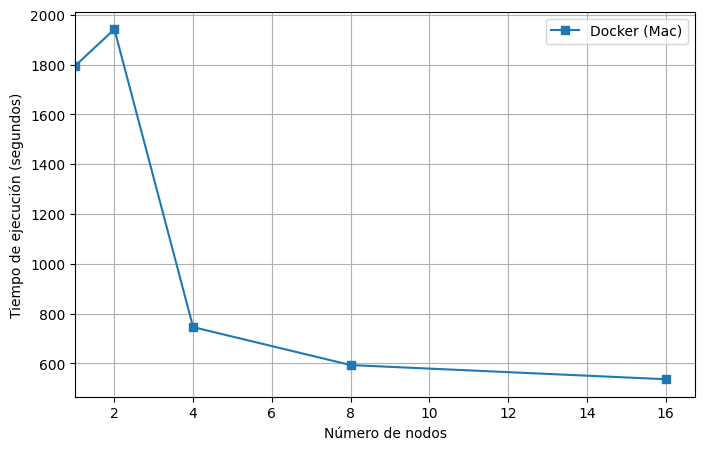
\includegraphics[width=0.8\textwidth]{imagenes/cap5/multi-node_mac_docker_time.png}
    \caption{Tiempo de ejecución en función del número de hebras en contenedores de Mac (CPU) en entorno multiproceso.}
    \label{fig:multi-node_mac_docker_time}
\end{figure}

En la tabla \ref{tab:multi-node_mac_docker} se presentan los tiempos de ejecución y la reducción porcentual respecto a una hebra.

\begin{table}[ht]
    \centering
    \begin{tabular}{|c|c|c|}
        \hline
        \textbf{Procesos} & \textbf{Tiempo (s)} & \textbf{$\Delta$\% vs 1 proceso} \\
        \hline
        1.00              & 1794.98             & 0.00                             \\
        2.00              & 1942.42             & 8.21                             \\
        4.00              & 745.84              & -58.45                           \\
        8.00              & 593.47              & -66.94                           \\
        16.00             & 536.60              & -70.11                           \\
        \hline
    \end{tabular}
    \caption{Tiempos de ejecución y reducción porcentual respecto a un proceso en entorno multiproceso con contenedores de Mac (CPU).}
    \label{tab:multi-node_mac_docker}
\end{table}

La tabla muestra la evolución del tiempo de ejecución al aumentar el número de procesos en un entorno multiproceso con contenedores de \textit{Docker} sobre Mac utilizando CPU. Con un solo proceso, se establece el tiempo de referencia. Al pasar a dos procesos, se observa un incremento del 8.21\% en el tiempo de ejecución, lo que indica que la paralelización inicial introduce una penalización, probablemente debida a la sobrecarga de coordinación o a limitaciones en la gestión de recursos en el entorno de contenedores sobre Mac. Sin embargo, al aumentar a cuatro procesos, el tiempo de ejecución disminuye de manera significativa, con una reducción del 58.45\%, lo que evidencia una mejora notable en el rendimiento gracias a la paralelización. Esta tendencia positiva se mantiene al escalar a ocho y dieciséis procesos, donde las reducciones alcanzan el 66.94\% y el 70.11\% respectivamente, mostrando que el sistema es capaz de aprovechar de manera eficiente los recursos adicionales a medida que se incrementa el número de procesos. En conjunto, los resultados indican que, aunque existe una penalización inicial al duplicar los procesos, el entorno multiproceso con contenedores de \textit{Docker} en Mac logra una escalabilidad efectiva y una mejora sustancial del rendimiento a partir de cuatro procesos, confirmando la viabilidad de esta tecnología para la ejecución de aplicaciones paralelas en este contexto.

En la figura \ref{fig:multi-node_mac_podman_time} se muestra el tiempo de ejecución para la configuración de CPU en un entorno multiproceso con contenedores de \textit{Podman} en Mac.

\begin{figure}[H]
    \centering
    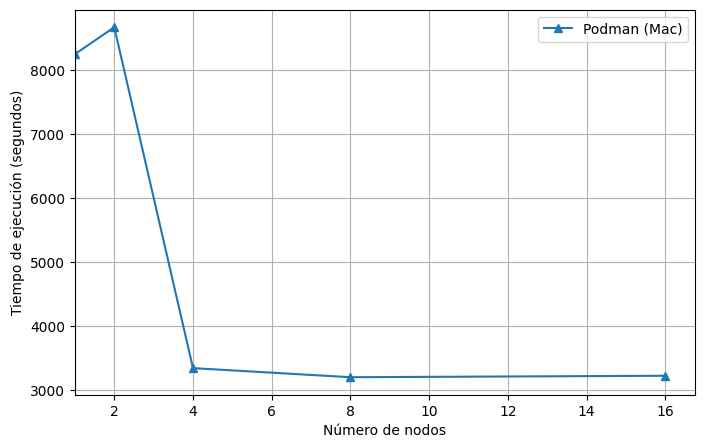
\includegraphics[width=0.8\textwidth]{imagenes/cap5/multi-node_mac_podman_time.png}
    \caption{Tiempo de ejecución en función del número de hebras en contenedores de \textit{Podman} (CPU) en entorno multiproceso.}
    \label{fig:multi-node_mac_podman_time}
\end{figure}

En la tabla \ref{tab:multi-node_mac_podman} se presentan los tiempos de ejecución y la reducción porcentual respecto a una hebra.

\begin{table}[ht]
    \centering
    \begin{tabular}{|c|c|c|}
        \hline
        \textbf{Procesos} & \textbf{Tiempo (s)} & \textbf{$\Delta$\% vs 1 proceso} \\
        \hline
        1.00              & 8247.00             & 0.00                             \\
        2.00              & 8668.00             & 5.10                             \\
        4.00              & 3343.15             & -59.46                           \\
        8.00              & 3201.07             & -61.19                           \\
        16.00             & 3223.98             & -60.91                           \\
        \hline
    \end{tabular}
    \caption{Tiempos de ejecución y reducción porcentual respecto a un proceso en entorno multiproceso con contenedores de \textit{Podman} en Mac (CPU).}
    \label{tab:multi-node_mac_podman}
\end{table}

La tabla muestra la evolución del tiempo de ejecución al aumentar el número de procesos en un entorno multiproceso con contenedores de \textit{Podman} sobre Mac utilizando CPU. Con un solo proceso, el tiempo de ejecución es el más alto y sirve como referencia. Al pasar a dos procesos, se observa un incremento del 5.10\% en el tiempo de ejecución, lo que indica que la paralelización inicial introduce una penalización, probablemente relacionada con la sobrecarga de coordinación o limitaciones en la gestión de recursos en este entorno. Sin embargo, al aumentar a cuatro procesos, el tiempo de ejecución disminuye de manera muy significativa, con una reducción del 59.46\%, lo que refleja una mejora notable en el rendimiento gracias a la paralelización. Esta mejora se mantiene al escalar a ocho y dieciséis procesos, donde las reducciones se sitúan en torno al 61\%, mostrando que el sistema es capaz de aprovechar de manera eficiente los recursos adicionales a partir de cuatro procesos. En conjunto, los resultados indican que, aunque existe una penalización inicial al duplicar los procesos, el entorno multiproceso con contenedores de \textit{Podman} en Mac logra una escalabilidad efectiva y una mejora sustancial del rendimiento a partir de cuatro procesos, confirmando la viabilidad de esta tecnología para la ejecución de aplicaciones paralelas en este contexto.

\section{Pruebas de barrido de hebras}
\subsection{Ejecución en Ubuntu en nativo}
\subsubsection{CPU}

En la figura \ref{fig:thread_sweep_ubuntu_cpu_native_time} se muestra el tiempo de ejecución para la configuración de CPU en un entorno nativo con Ubuntu.

\begin{figure}[H]
    \centering
    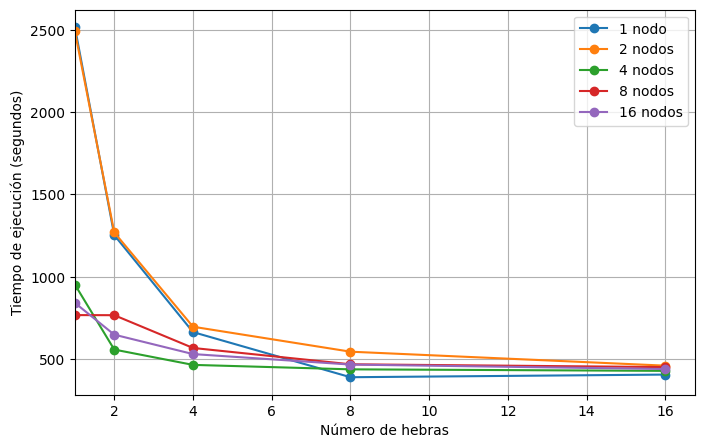
\includegraphics[width=0.8\textwidth]{imagenes/cap5/thread_sweep_ubuntu_cpu_native_time.png}
    \caption{Tiempo de ejecución en función del número de hebras en entorno nativo de Ubuntu (CPU).}
    \label{fig:thread_sweep_ubuntu_cpu_native_time}
\end{figure}

En la tabla \ref{tab:thread_sweep_ubuntu_cpu_native} se presentan los tiempos de ejecución y la reducción porcentual respecto a una hebra.

\begin{table}[ht]
    \centering
    \begin{tabular}{|c|c|c|c|}
        \hline
        \textbf{Procesos} & \textbf{Hebras} & \textbf{Tiempo (s)} & \textbf{$\Delta$\% vs 1 hebra} \\
        \hline
        1.00              & 1.00            & 2515.21             & 0.00                           \\
        1.00              & 2.00            & 1253.18             & -50.18                         \\
        1.00              & 4.00            & 664.69              & -73.57                         \\
        1.00              & 8.00            & 390.72              & -84.47                         \\
        1.00              & 16.00           & 406.76              & -83.83                         \\
        2.00              & 1.00            & 2489.49             & 0.00                           \\
        2.00              & 2.00            & 1269.36             & -49.01                         \\
        2.00              & 4.00            & 697.22              & -71.99                         \\
        2.00              & 8.00            & 545.73              & -78.08                         \\
        2.00              & 16.00           & 460.89              & -81.49                         \\
        4.00              & 1.00            & 952.85              & 0.00                           \\
        4.00              & 2.00            & 558.59              & -41.38                         \\
        4.00              & 4.00            & 465.64              & -51.13                         \\
        4.00              & 8.00            & 438.55              & -53.97                         \\
        4.00              & 16.00           & 429.30              & -54.95                         \\
        8.00              & 1.00            & 767.87              & 0.00                           \\
        8.00              & 2.00            & 767.21              & -0.09                          \\
        8.00              & 4.00            & 568.34              & -25.98                         \\
        8.00              & 8.00            & 469.23              & -38.89                         \\
        8.00              & 16.00           & 452.19              & -41.11                         \\
        16.00             & 1.00            & 841.96              & 0.00                           \\
        16.00             & 2.00            & 649.02              & -22.92                         \\
        16.00             & 4.00            & 531.22              & -36.91                         \\
        16.00             & 8.00            & 467.56              & -44.47                         \\
        16.00             & 16.00           & 440.44              & -47.69                         \\
        \hline
    \end{tabular}
    \caption{Tiempos de ejecución y reducción porcentual respecto a una hebra para distintas combinaciones de procesos y hebras en entorno nativo de Ubuntu (CPU).}
    \label{tab:thread_sweep_ubuntu_cpu_native}
\end{table}

La tabla recoge los tiempos de ejecución y la reducción porcentual respecto a una hebra para distintas combinaciones de procesos y hebras en un entorno nativo de Ubuntu utilizando CPU. Al analizar los resultados, se observa que el mayor beneficio en la reducción del tiempo de ejecución se obtiene al incrementar el número de hebras en configuraciones de un solo proceso, alcanzando una reducción del 84.47\% con ocho hebras respecto a la ejecución secuencial. Sin embargo, al aumentar a dieciséis hebras, el tiempo de ejecución apenas mejora e incluso empeora ligeramente, lo que sugiere que el paralelismo óptimo se alcanza en torno a ocho hebras, probablemente coincidiendo con el número de núcleos físicos disponibles. Cuando se incrementa el número de procesos, la reducción porcentual respecto a una hebra disminuye progresivamente, y el beneficio de añadir más hebras es cada vez menor. Por ejemplo, con dieciséis procesos y dieciséis hebras, la reducción es del 47.69\%, muy inferior a la obtenida en el caso monoproceso. Esto indica que la sobrecarga de coordinación y comunicación entre procesos limita la eficiencia del paralelismo a medida que se incrementa el número de procesos, haciendo que el escalado no sea lineal. En resumen, el entorno nativo de Ubuntu permite un aprovechamiento muy eficiente del paralelismo en configuraciones monoproceso, pero la eficiencia disminuye al aumentar el número de procesos, especialmente cuando se superan los límites físicos de la arquitectura o se incrementa la complejidad de la comunicación entre procesos.

En la figura \ref{fig:thread_sweep_ubuntu_cpu_native_cpu} se muestra el uso de CPU para la configuración de CPU en un entorno nativo con Ubuntu.

\begin{figure}[H]
    \centering
    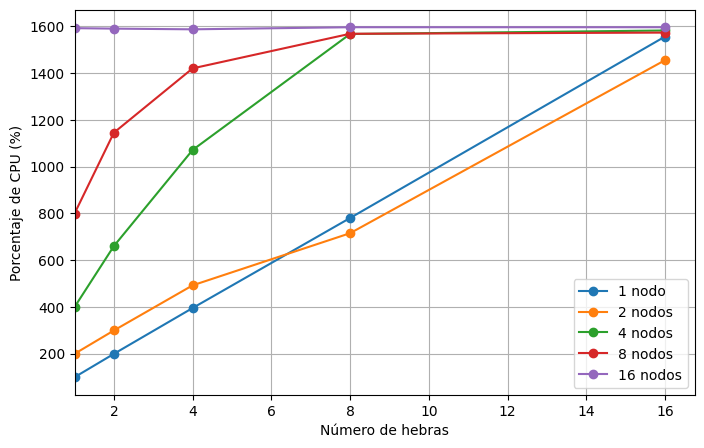
\includegraphics[width=0.8\textwidth]{imagenes/cap5/thread_sweep_ubuntu_cpu_native_cpu.png}
    \caption{Uso de CPU en función del número de hebras en entorno nativo de Ubuntu (CPU).}
    \label{fig:thread_sweep_ubuntu_cpu_native_cpu}
\end{figure}

En la tabla \ref{tab:thread_sweep_ubuntu_cpu_native_cpu} se presentan los valores de uso de CPU para distintas combinaciones de procesos y hebras.

\begin{table}[ht]
    \centering
    \begin{tabular}{|c|c|c|c|c|}
        \hline
        \textbf{Procesos} & \textbf{Hebras} & \textbf{CPU (\%)} & \textbf{Max (\%)} & \textbf{Efic. (\%)} \\
        \hline
        1.00              & 1.00            & 99.00             & 100.00            & 99.00               \\
        1.00              & 2.00            & 199.00            & 200.00            & 99.50               \\
        1.00              & 4.00            & 395.00            & 400.00            & 98.75               \\
        1.00              & 8.00            & 780.00            & 800.00            & 97.50               \\
        1.00              & 16.00           & 1556.00           & 1600.00           & 97.25               \\
        2.00              & 1.00            & 199.00            & 100.00            & 199.00              \\
        2.00              & 2.00            & 299.00            & 200.00            & 149.50              \\
        2.00              & 4.00            & 492.00            & 400.00            & 123.00              \\
        2.00              & 8.00            & 715.00            & 800.00            & 89.38               \\
        2.00              & 16.00           & 1455.00           & 1600.00           & 90.94               \\
        4.00              & 1.00            & 399.00            & 100.00            & 399.00              \\
        4.00              & 2.00            & 660.00            & 200.00            & 330.00              \\
        4.00              & 4.00            & 1071.00           & 400.00            & 267.75              \\
        4.00              & 8.00            & 1567.00           & 800.00            & 195.88              \\
        4.00              & 16.00           & 1582.00           & 1600.00           & 98.88               \\
        8.00              & 1.00            & 799.00            & 100.00            & 799.00              \\
        8.00              & 2.00            & 1145.00           & 200.00            & 572.50              \\
        8.00              & 4.00            & 1420.00           & 400.00            & 355.00              \\
        8.00              & 8.00            & 1568.00           & 800.00            & 196.00              \\
        8.00              & 16.00           & 1573.00           & 1600.00           & 98.31               \\
        16.00             & 1.00            & 1592.00           & 100.00            & 1592.00             \\
        16.00             & 2.00            & 1590.00           & 200.00            & 795.00              \\
        16.00             & 4.00            & 1587.00           & 400.00            & 396.75              \\
        16.00             & 8.00            & 1596.00           & 800.00            & 199.50              \\
        16.00             & 16.00           & 1596.00           & 1600.00           & 99.75               \\
        \hline
    \end{tabular}
    \caption{Valores de uso de CPU, máximo teórico y eficiencia para distintas combinaciones de procesos y hebras en entorno nativo de Ubuntu (CPU).}
    \label{tab:thread_sweep_ubuntu_cpu_native_cpu}
\end{table}

La tabla recoge el porcentaje de uso de CPU, el máximo teórico posible y la eficiencia alcanzada para diferentes combinaciones de procesos y hebras en un entorno nativo de Ubuntu. Cuando se utiliza un solo proceso, el uso de CPU crece de forma casi lineal con el número de hebras y la eficiencia se mantiene muy alta, siempre por encima del 97\%, lo que indica un excelente aprovechamiento de los recursos disponibles y una sobrecarga mínima asociada a la gestión de los hilos. Al aumentar el número de procesos, el uso total de CPU también crece, pero la eficiencia relativa disminuye de manera progresiva, especialmente cuando el número de hebras por proceso es bajo. Por ejemplo, con dos procesos y una hebra, la eficiencia es del 199\%, reflejando que se suman los recursos de ambos procesos, pero a medida que se incrementa el número de hebras, la eficiencia cae, situándose en torno al 90\% con dieciséis hebras. Este patrón se repite y se acentúa al escalar a cuatro, ocho y dieciséis procesos, donde la eficiencia solo se mantiene cercana al 100\% cuando el número de hebras por proceso es máximo. En configuraciones con muchos procesos y pocas hebras, la eficiencia es baja, lo que evidencia que la sobrecarga de coordinación y la distribución de tareas penalizan el aprovechamiento de los recursos. Sin embargo, cuando se asigna el máximo número de hebras por proceso, la eficiencia vuelve a valores cercanos al 100\%, lo que sugiere que el sistema es capaz de escalar eficazmente siempre que se maximice el paralelismo interno de cada proceso. En conjunto, estos resultados muestran que el entorno nativo de Ubuntu permite un uso muy eficiente de la CPU en configuraciones monoproceso y que, en escenarios multiproceso, la eficiencia depende en gran medida de la relación entre el número de procesos y el número de hebras asignadas a cada uno.

\subsubsection{CPU + GPU}

En la figura \ref{fig:thread_sweep_ubuntu_gpu_native_time} se muestra el tiempo de ejecución para la configuración de CPU + GPU en un entorno nativo con Ubuntu.

\begin{figure}[H]
    \centering
    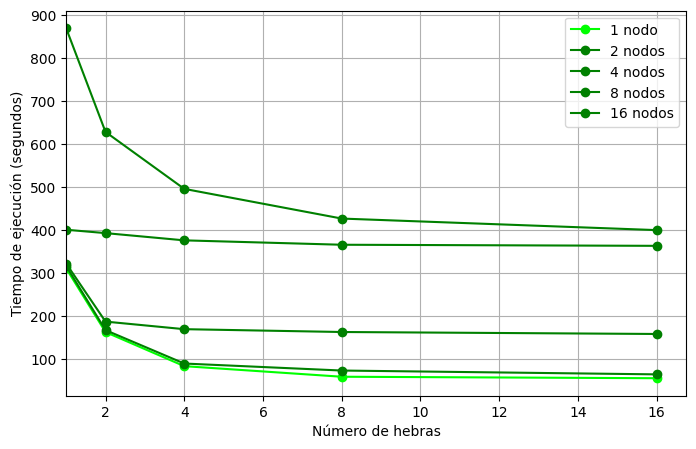
\includegraphics[width=0.8\textwidth]{imagenes/cap5/thread_sweep_ubuntu_gpu_native_time.png}
    \caption{Tiempo de ejecución en función del número de hebras en entorno nativo de Ubuntu (CPU + GPU).}
    \label{fig:thread_sweep_ubuntu_gpu_native_time}
\end{figure}

En la tabla \ref{tab:thread_sweep_ubuntu_gpu_native} se presentan los tiempos de ejecución y la reducción porcentual respecto a una hebra.

\begin{table}[ht]
    \centering
    \begin{tabular}{|c|c|c|c|}
        \hline
        \textbf{Procesos} & \textbf{Hebras} & \textbf{Tiempo (s)} & \textbf{$\Delta$\% vs 1 hebra} \\
        \hline
        1.00              & 1.00            & 311.68              & 0.00                           \\
        1.00              & 2.00            & 163.59              & -47.51                         \\
        1.00              & 4.00            & 84.49               & -72.89                         \\
        1.00              & 8.00            & 59.91               & -80.78                         \\
        1.00              & 16.00           & 56.45               & -81.89                         \\
        2.00              & 1.00            & 316.92              & 0.00                           \\
        2.00              & 2.00            & 168.14              & -46.95                         \\
        2.00              & 4.00            & 90.58               & -71.42                         \\
        2.00              & 8.00            & 74.30               & -76.56                         \\
        2.00              & 16.00           & 65.40               & -79.36                         \\
        4.00              & 1.00            & 322.77              & 0.00                           \\
        4.00              & 2.00            & 187.98              & -41.76                         \\
        4.00              & 4.00            & 170.38              & -47.21                         \\
        4.00              & 8.00            & 163.80              & -49.25                         \\
        4.00              & 16.00           & 159.22              & -50.67                         \\
        8.00              & 1.00            & 401.33              & 0.00                           \\
        8.00              & 2.00            & 393.50              & -1.95                          \\
        8.00              & 4.00            & 376.68              & -6.14                          \\
        8.00              & 8.00            & 366.47              & -8.69                          \\
        8.00              & 16.00           & 363.94              & -9.32                          \\
        16.00             & 1.00            & 869.40              & 0.00                           \\
        16.00             & 2.00            & 628.49              & -27.71                         \\
        16.00             & 4.00            & 496.28              & -42.92                         \\
        16.00             & 8.00            & 427.30              & -50.85                         \\
        16.00             & 16.00           & 400.48              & -53.94                         \\
        \hline
    \end{tabular}
    \caption{Tiempos de ejecución y reducción porcentual respecto a una hebra para distintas combinaciones de procesos y hebras en entorno nativo de Ubuntu (CPU + GPU).}
    \label{tab:thread_sweep_ubuntu_gpu_native}
\end{table}

La tabla recoge los tiempos de ejecución y la reducción porcentual respecto a una hebra para distintas combinaciones de procesos y hebras en un entorno nativo de Ubuntu utilizando CPU y GPU. Al analizar los resultados, se observa que el mayor beneficio en la reducción del tiempo de ejecución se obtiene al incrementar el número de hebras en configuraciones de un solo proceso, alcanzando una reducción del 81.89\% con dieciséis hebras respecto a la ejecución secuencial. El descenso del tiempo es especialmente acusado al pasar de una a dos hebras y de dos a cuatro, mientras que a partir de ocho hebras la mejora adicional es más limitada, lo que indica que el paralelismo óptimo se alcanza en torno a ese valor y que el sistema comienza a saturarse. Cuando se incrementa el número de procesos, la reducción porcentual respecto a una hebra disminuye progresivamente y el beneficio de añadir más hebras es cada vez menor. Por ejemplo, con dieciséis procesos y dieciséis hebras, la reducción es del 53.94\%, muy inferior a la obtenida en el caso monoproceso. Además, en configuraciones con ocho procesos o más, el incremento de hebras apenas aporta mejoras, lo que sugiere que la sobrecarga de coordinación y la gestión de la GPU entre procesos limita la eficiencia del paralelismo. En resumen, la combinación de CPU y GPU permite un aprovechamiento muy eficiente del paralelismo en configuraciones monoproceso, pero la eficiencia disminuye al aumentar el número de procesos, especialmente cuando se incrementa la complejidad de la comunicación y la gestión de recursos compartidos.

En la figura \ref{fig:thread_sweep_ubuntu_gpu_native_cpu} se muestra el uso de CPU para la configuración de CPU + GPU en un entorno nativo con Ubuntu.

\begin{figure}[H]
    \centering
    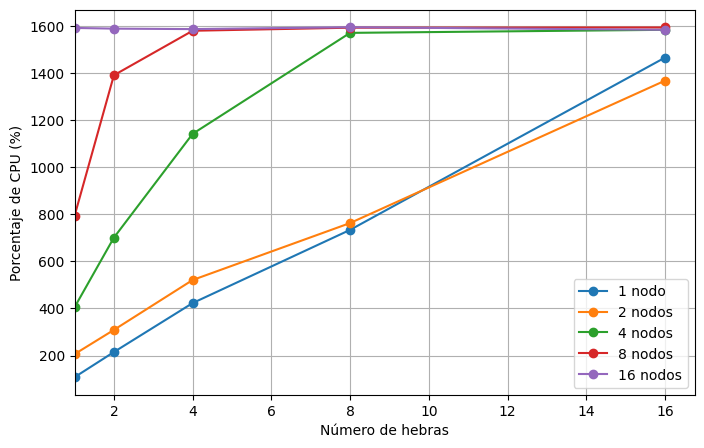
\includegraphics[width=0.8\textwidth]{imagenes/cap5/thread_sweep_ubuntu_gpu_native_cpu.png}
    \caption{Uso de CPU en función del número de hebras en entorno nativo de Ubuntu (CPU + GPU).}
    \label{fig:thread_sweep_ubuntu_gpu_native_cpu}
\end{figure}

En la tabla \ref{tab:thread_sweep_ubuntu_gpu_native_cpu} se presentan los valores de uso de CPU para distintas combinaciones de procesos y hebras.

\begin{table}[ht]
    \centering
    \begin{tabular}{|c|c|c|c|c|}
        \hline
        \textbf{Procesos} & \textbf{Hebras} & \textbf{CPU (\%)} & \textbf{Max (\%)} & \textbf{Efic. (\%)} \\
        \hline
        1.00              & 1.00            & 108.00            & 100.00            & 108.00              \\
        1.00              & 2.00            & 215.00            & 200.00            & 107.50              \\
        1.00              & 4.00            & 423.00            & 400.00            & 105.75              \\
        1.00              & 8.00            & 734.00            & 800.00            & 91.75               \\
        1.00              & 16.00           & 1466.00           & 1600.00           & 91.62               \\
        2.00              & 1.00            & 206.00            & 100.00            & 206.00              \\
        2.00              & 2.00            & 309.00            & 200.00            & 154.50              \\
        2.00              & 4.00            & 521.00            & 400.00            & 130.25              \\
        2.00              & 8.00            & 763.00            & 800.00            & 95.38               \\
        2.00              & 16.00           & 1368.00           & 1600.00           & 85.50               \\
        4.00              & 1.00            & 405.00            & 100.00            & 405.00              \\
        4.00              & 2.00            & 701.00            & 200.00            & 350.50              \\
        4.00              & 4.00            & 1142.00           & 400.00            & 285.50              \\
        4.00              & 8.00            & 1571.00           & 800.00            & 196.38              \\
        4.00              & 16.00           & 1584.00           & 1600.00           & 99.00               \\
        8.00              & 1.00            & 793.00            & 100.00            & 793.00              \\
        8.00              & 2.00            & 1391.00           & 200.00            & 695.50              \\
        8.00              & 4.00            & 1580.00           & 400.00            & 395.00              \\
        8.00              & 8.00            & 1593.00           & 800.00            & 199.12              \\
        8.00              & 16.00           & 1594.00           & 1600.00           & 99.62               \\
        16.00             & 1.00            & 1592.00           & 100.00            & 1592.00             \\
        16.00             & 2.00            & 1589.00           & 200.00            & 794.50              \\
        16.00             & 4.00            & 1587.00           & 400.00            & 396.75              \\
        16.00             & 8.00            & 1595.00           & 800.00            & 199.38              \\
        16.00             & 16.00           & 1584.00           & 1600.00           & 99.00               \\
        \hline
    \end{tabular}
    \caption{Valores de uso de CPU, uso máximo teórico y eficiencia para distintas combinaciones de procesos y hebras en entorno nativo de Ubuntu (CPU + GPU).}
    \label{tab:thread_sweep_ubuntu_gpu_native_cpu}
\end{table}

La tabla presenta los valores de uso de CPU, el máximo teórico y la eficiencia para diferentes combinaciones de procesos y hebras en un entorno nativo de Ubuntu utilizando CPU y GPU. En configuraciones monoproceso, el porcentaje de uso de CPU supera el 100\% en todos los casos, lo que refleja la contribución de la GPU al cómputo total y explica que la eficiencia calculada también supere el 100\% para valores bajos de hebras. A medida que se incrementa el número de hebras, la eficiencia disminuye ligeramente, situándose en torno al 91\% con 8 y 16 hebras, lo que indica que el sistema sigue aprovechando bien los recursos, aunque la saturación y la sobrecarga empiezan a notarse.

Al aumentar el número de procesos, el uso total de CPU crece de forma proporcional, pero la eficiencia relativa desciende de manera más acusada cuando el número de hebras por proceso es bajo, alcanzando valores muy elevados (por encima del 200\% o incluso del 700\% en algunos casos) debido a la suma de recursos de CPU y GPU en todos los procesos. Sin embargo, a medida que se incrementa el número de hebras, la eficiencia tiende a estabilizarse en torno al 99\% cuando se alcanza el máximo teórico de uso de CPU, lo que indica que el sistema es capaz de escalar eficazmente siempre que se maximice el paralelismo interno de cada proceso.

En conjunto, estos resultados muestran que la combinación de CPU y GPU permite un uso muy eficiente de los recursos en configuraciones monoproceso y que, en escenarios multiproceso, la eficiencia depende de la relación entre el número de procesos y el número de hebras asignadas, siendo óptima cuando se aprovechan al máximo las capacidades de cómputo de cada proceso.

% \subsubsection{Comparativa de rendimiento CPU vs CPU + GPU}

\subsection{Ejecución en contenedores de Ubuntu}
\subsubsection{CPU}

En la figura \ref{fig:thread_sweep_ubuntu_docker_time} se muestra el tiempo de ejecución para la configuración de CPU en un entorno con contenedores de Ubuntu.

\begin{figure}[H]
    \centering
    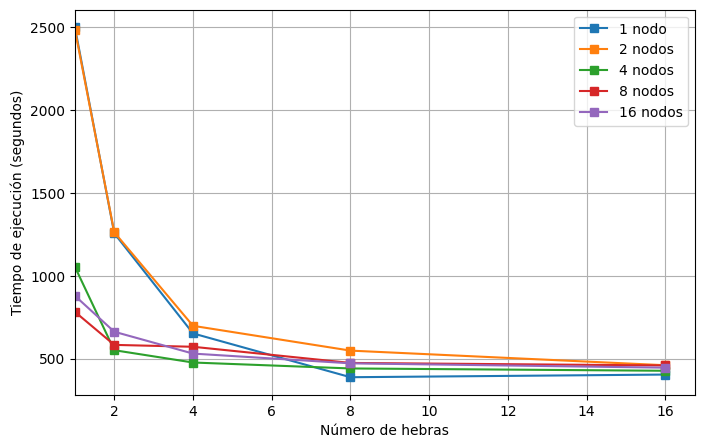
\includegraphics[width=0.8\textwidth]{imagenes/cap5/thread_sweep_ubuntu_docker_time.png}
    \caption{Tiempo de ejecución en función del número de hebras en contenedores de Ubuntu (CPU).}
    \label{fig:thread_sweep_ubuntu_docker_time}
\end{figure}

En la tabla \ref{tab:thread_sweep_ubuntu_docker_time} se presentan los tiempos de ejecución y la reducción porcentual respecto a una hebra.

\begin{table}[ht]
    \centering
    \begin{tabular}{|c|c|c|c|}
        \hline
        \textbf{Procesos} & \textbf{Hebras} & \textbf{Tiempo (s)} & \textbf{$\Delta$\% vs 1 hebra} \\
        \hline
        1.00              & 1.00            & 2499.09             & 0.00                           \\
        1.00              & 2.00            & 1255.95             & -49.74                         \\
        1.00              & 4.00            & 652.33              & -73.90                         \\
        1.00              & 8.00            & 388.04              & -84.47                         \\
        1.00              & 16.00           & 404.09              & -83.83                         \\
        2.00              & 1.00            & 2484.80             & 0.00                           \\
        2.00              & 2.00            & 1262.23             & -49.20                         \\
        2.00              & 4.00            & 698.05              & -71.91                         \\
        2.00              & 8.00            & 548.49              & -77.93                         \\
        2.00              & 16.00           & 460.29              & -81.48                         \\
        4.00              & 1.00            & 1054.20             & 0.00                           \\
        4.00              & 2.00            & 551.03              & -47.73                         \\
        4.00              & 4.00            & 476.76              & -54.78                         \\
        4.00              & 8.00            & 440.94              & -58.17                         \\
        4.00              & 16.00           & 426.96              & -59.50                         \\
        8.00              & 1.00            & 782.42              & 0.00                           \\
        8.00              & 2.00            & 583.08              & -25.48                         \\
        8.00              & 4.00            & 571.72              & -26.93                         \\
        8.00              & 8.00            & 474.19              & -39.39                         \\
        8.00              & 16.00           & 459.06              & -41.33                         \\
        16.00             & 1.00            & 879.20              & 0.00                           \\
        16.00             & 2.00            & 662.38              & -24.66                         \\
        16.00             & 4.00            & 530.59              & -39.65                         \\
        16.00             & 8.00            & 471.83              & -46.33                         \\
        16.00             & 16.00           & 445.63              & -49.31                         \\
        \hline
    \end{tabular}
    \caption{Tiempos de ejecución y reducción porcentual respecto a una hebra para distintas combinaciones de procesos y hebras en contenedores de Ubuntu (CPU).}
    \label{tab:thread_sweep_ubuntu_docker_time}
\end{table}

La tabla muestra los tiempos de ejecución y la reducción porcentual respecto a una hebra para distintas combinaciones de procesos y hebras en contenedores de Ubuntu utilizando CPU. Se observa que, en configuraciones monoproceso, el incremento del número de hebras produce una reducción muy significativa del tiempo de ejecución, alcanzando una disminución del 84.47\% con ocho hebras respecto a la ejecución secuencial. Sin embargo, al aumentar a dieciséis hebras, el tiempo de ejecución apenas mejora e incluso empeora ligeramente, lo que indica que el paralelismo óptimo se sitúa en torno a ocho hebras, probablemente coincidiendo con el número de núcleos físicos disponibles. Al incrementar el número de procesos, la reducción porcentual respecto a una hebra disminuye progresivamente y el beneficio de añadir más hebras es cada vez menor. Por ejemplo, con dieciséis procesos y dieciséis hebras, la reducción es del 49.31\%, notablemente inferior a la obtenida en el caso monoproceso. Además, en configuraciones con muchos procesos, el incremento de hebras aporta mejoras más limitadas, lo que sugiere que la sobrecarga de coordinación y la gestión de recursos entre contenedores penalizan la eficiencia del paralelismo. En conjunto, el entorno con contenedores de Ubuntu permite un aprovechamiento eficiente del paralelismo en configuraciones monoproceso, pero la eficiencia disminuye al aumentar el número de procesos, especialmente cuando se incrementa la complejidad de la comunicación y la gestión de procesos distribuidos.

En la figura \ref{fig:thread_sweep_ubuntu_podman_time} se muestra el tiempo de ejecución para la configuración de CPU en un entorno con contenedores de \textit{Podman}.

\begin{figure}[H]
    \centering
    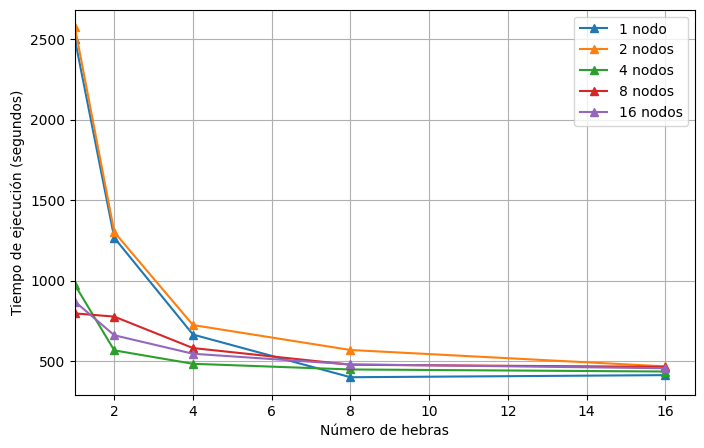
\includegraphics[width=0.8\textwidth]{imagenes/cap5/thread_sweep_ubuntu_podman_time.png}
    \caption{Tiempo de ejecución en función del número de hebras en contenedores de \textit{Podman} (CPU).}
    \label{fig:thread_sweep_ubuntu_podman_time}
\end{figure}

En la tabla \ref{tab:thread_sweep_ubuntu_podman_time} se presentan los tiempos de ejecución y la reducción porcentual respecto a una hebra.

\begin{table}[ht]
    \centering
    \begin{tabular}{|c|c|c|c|}
        \hline
        \textbf{Procesos} & \textbf{Hebras} & \textbf{Tiempo (s)} & \textbf{$\Delta$\% vs 1 hebra} \\
        \hline
        1.00              & 1.00            & 2499.16             & 0.00                           \\
        1.00              & 2.00            & 1266.51             & -49.32                         \\
        1.00              & 4.00            & 665.38              & -73.38                         \\
        1.00              & 8.00            & 400.51              & -83.97                         \\
        1.00              & 16.00           & 413.53              & -83.45                         \\
        2.00              & 1.00            & 2574.04             & 0.00                           \\
        2.00              & 2.00            & 1301.72             & -49.43                         \\
        2.00              & 4.00            & 724.50              & -71.85                         \\
        2.00              & 8.00            & 569.61              & -77.87                         \\
        2.00              & 16.00           & 467.63              & -81.83                         \\
        4.00              & 1.00            & 973.92              & 0.00                           \\
        4.00              & 2.00            & 567.28              & -41.75                         \\
        4.00              & 4.00            & 483.88              & -50.32                         \\
        4.00              & 8.00            & 448.66              & -53.93                         \\
        4.00              & 16.00           & 435.93              & -55.24                         \\
        8.00              & 1.00            & 796.84              & 0.00                           \\
        8.00              & 2.00            & 776.89              & -2.50                          \\
        8.00              & 4.00            & 581.62              & -27.01                         \\
        8.00              & 8.00            & 477.89              & -40.03                         \\
        8.00              & 16.00           & 464.91              & -41.66                         \\
        16.00             & 1.00            & 870.28              & 0.00                           \\
        16.00             & 2.00            & 661.10              & -24.04                         \\
        16.00             & 4.00            & 546.24              & -37.23                         \\
        16.00             & 8.00            & 480.46              & -44.79                         \\
        16.00             & 16.00           & 456.25              & -47.57                         \\
        \hline
    \end{tabular}
    \caption{Tiempos de ejecución y reducción porcentual respecto a una hebra para distintas combinaciones de procesos y hebras en contenedores de \textit{Podman} (CPU).}
    \label{tab:thread_sweep_ubuntu_podman_time}
\end{table}

La tabla recoge los tiempos de ejecución y la reducción porcentual respecto a una hebra para distintas combinaciones de procesos y hebras en contenedores de \textit{Podman} utilizando CPU. En configuraciones monoproceso, el incremento del número de hebras produce una reducción muy significativa del tiempo de ejecución, alcanzando una disminución del 83.97\% con ocho hebras respecto a la ejecución secuencial. Sin embargo, al aumentar a dieciséis hebras, el tiempo de ejecución apenas mejora e incluso empeora ligeramente, lo que indica que el paralelismo óptimo se sitúa en torno a ocho hebras, probablemente coincidiendo con el número de núcleos físicos disponibles. Al incrementar el número de procesos, la reducción porcentual respecto a una hebra disminuye progresivamente y el beneficio de añadir más hebras es cada vez menor. Por ejemplo, con dieciséis procesos y dieciséis hebras, la reducción es del 47.57\%, notablemente inferior a la obtenida en el caso monoproceso. Además, en configuraciones con muchos procesos, el incremento de hebras aporta mejoras más limitadas, lo que sugiere que la sobrecarga de coordinación y la gestión de recursos entre contenedores penalizan la eficiencia del paralelismo. En conjunto, el entorno con contenedores de \textit{Podman} permite un aprovechamiento eficiente del paralelismo en configuraciones monoproceso, pero la eficiencia disminuye al aumentar el número de procesos, especialmente cuando se incrementa la complejidad de la comunicación y la gestión de procesos distribuidos.

\subsubsection{CPU + GPU}

En la figura \ref{fig:thread_sweep_ubuntu_docker_gpu_time} se muestra el tiempo de ejecución para la configuración de CPU + GPU en un entorno con contenedores de Ubuntu.

\begin{figure}[H]
    \centering
    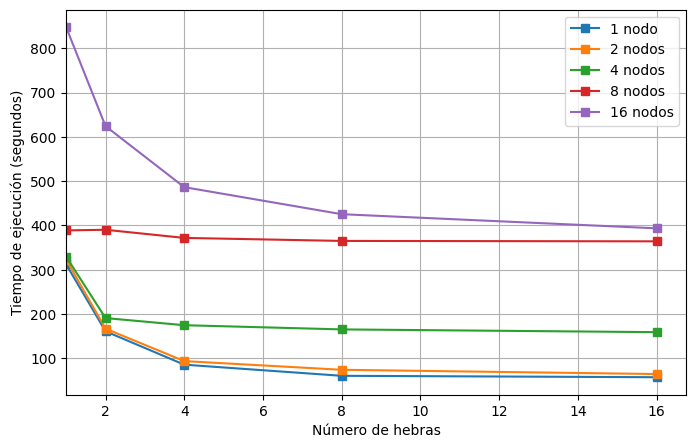
\includegraphics[width=0.8\textwidth]{imagenes/cap5/thread_sweep_ubuntu_docker_gpu_time.png}
    \caption{Tiempo de ejecución en función del número de hebras en contenedores de Ubuntu (CPU + GPU).}
    \label{fig:thread_sweep_ubuntu_docker_gpu_time}
\end{figure}

En la tabla \ref{tab:thread_sweep_ubuntu_docker_gpu_time} se presentan los tiempos de ejecución y la reducción porcentual respecto a una hebra.

\begin{table}[ht]
    \centering
    \begin{tabular}{|c|c|c|c|}
        \hline
        \textbf{Procesos} & \textbf{Hebras} & \textbf{Tiempo (s)} & \textbf{$\Delta$\% vs 1 hebra} \\
        \hline
        1.00              & 1.00            & 312.18              & 0.00                           \\
        1.00              & 2.00            & 161.10              & -48.40                         \\
        1.00              & 4.00            & 85.78               & -72.52                         \\
        1.00              & 8.00            & 60.65               & -80.57                         \\
        1.00              & 16.00           & 57.45               & -81.60                         \\
        2.00              & 1.00            & 322.77              & 0.00                           \\
        2.00              & 2.00            & 166.99              & -48.26                         \\
        2.00              & 4.00            & 93.85               & -70.92                         \\
        2.00              & 8.00            & 74.22               & -77.01                         \\
        2.00              & 16.00           & 64.60               & -79.99                         \\
        4.00              & 1.00            & 329.54              & 0.00                           \\
        4.00              & 2.00            & 190.95              & -42.06                         \\
        4.00              & 4.00            & 174.85              & -46.94                         \\
        4.00              & 8.00            & 165.36              & -49.82                         \\
        4.00              & 16.00           & 159.15              & -51.71                         \\
        8.00              & 1.00            & 388.78              & 0.00                           \\
        8.00              & 2.00            & 390.25              & 0.38                           \\
        8.00              & 4.00            & 371.88              & -4.35                          \\
        8.00              & 8.00            & 365.06              & -6.10                          \\
        8.00              & 16.00           & 364.13              & -6.34                          \\
        16.00             & 1.00            & 847.37              & 0.00                           \\
        16.00             & 2.00            & 624.14              & -26.34                         \\
        16.00             & 4.00            & 486.42              & -42.60                         \\
        16.00             & 8.00            & 425.37              & -49.80                         \\
        16.00             & 16.00           & 393.49              & -53.56                         \\
        \hline
    \end{tabular}
    \caption{Tiempos de ejecución y reducción porcentual respecto a una hebra para distintas combinaciones de procesos y hebras en contenedores \textit{Docker} de Ubuntu (CPU + GPU).}
    \label{tab:thread_sweep_ubuntu_docker_gpu_time}
\end{table}

La tabla recoge los tiempos de ejecución y la reducción porcentual respecto a una hebra para distintas combinaciones de procesos y hebras en contenedores de Ubuntu utilizando CPU y GPU. En configuraciones monoproceso, el incremento del número de hebras produce una reducción muy significativa del tiempo de ejecución, alcanzando una disminución del 81.60\% con dieciséis hebras respecto a la ejecución secuencial. El mayor beneficio se observa al pasar de una a dos hebras y de dos a cuatro, mientras que a partir de ocho hebras la mejora adicional es más limitada, lo que indica que el paralelismo óptimo se alcanza en torno a ese valor y que el sistema comienza a saturarse. Al aumentar el número de procesos, la reducción porcentual respecto a una hebra disminuye progresivamente y el beneficio de añadir más hebras es cada vez menor. Por ejemplo, con dieciséis procesos y dieciséis hebras, la reducción es del 53.56\%, notablemente inferior a la obtenida en el caso monoproceso. Además, en configuraciones con ocho procesos o más, el incremento de hebras apenas aporta mejoras, lo que sugiere que la sobrecarga de coordinación y la gestión de la GPU entre procesos limita la eficiencia del paralelismo. En conjunto, la combinación de CPU y GPU en contenedores de Ubuntu permite un aprovechamiento eficiente del paralelismo en configuraciones monoproceso, pero la eficiencia disminuye al aumentar el número de procesos, especialmente cuando se incrementa la complejidad de la comunicación y la gestión de recursos compartidos.

En la figura \ref{fig:thread_sweep_ubuntu_podman_gpu_time} se muestra el tiempo de ejecución para la configuración de CPU + GPU en un entorno con contenedores de \textit{Podman}.

\begin{figure}[H]
    \centering
    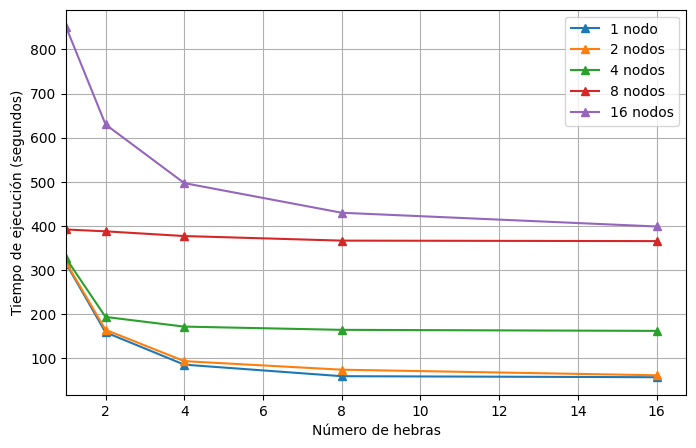
\includegraphics[width=0.8\textwidth]{imagenes/cap5/thread_sweep_ubuntu_podman_gpu_time.png}
    \caption{Tiempo de ejecución en función del número de hebras en contenedores de \textit{Podman} (CPU + GPU).}
    \label{fig:thread_sweep_ubuntu_podman_gpu_time}
\end{figure}

En la tabla \ref{tab:thread_sweep_ubuntu_podman_gpu_time} se presentan los tiempos de ejecución y la reducción porcentual respecto a una hebra.

\begin{table}[ht]
    \centering
    \begin{tabular}{|c|c|c|c|}
        \hline
        \textbf{Procesos} & \textbf{Hebras} & \textbf{Tiempo (s)} & \textbf{$\Delta$\% vs 1 hebra} \\
        \hline
        1.00              & 1.00            & 314.51              & 0.00                           \\
        1.00              & 2.00            & 158.84              & -49.50                         \\
        1.00              & 4.00            & 85.62               & -72.78                         \\
        1.00              & 8.00            & 59.47               & -81.09                         \\
        1.00              & 16.00           & 57.12               & -81.84                         \\
        2.00              & 1.00            & 316.80              & 0.00                           \\
        2.00              & 2.00            & 164.58              & -48.05                         \\
        2.00              & 4.00            & 93.56               & -70.47                         \\
        2.00              & 8.00            & 74.18               & -76.58                         \\
        2.00              & 16.00           & 61.51               & -80.58                         \\
        4.00              & 1.00            & 326.20              & 0.00                           \\
        4.00              & 2.00            & 193.69              & -40.62                         \\
        4.00              & 4.00            & 171.80              & -47.33                         \\
        4.00              & 8.00            & 164.47              & -49.58                         \\
        4.00              & 16.00           & 162.10              & -50.31                         \\
        8.00              & 1.00            & 391.86              & 0.00                           \\
        8.00              & 2.00            & 387.68              & -1.07                          \\
        8.00              & 4.00            & 377.01              & -3.79                          \\
        8.00              & 8.00            & 366.63              & -6.44                          \\
        8.00              & 16.00           & 365.54              & -6.72                          \\
        16.00             & 1.00            & 850.18              & 0.00                           \\
        16.00             & 2.00            & 629.92              & -25.91                         \\
        16.00             & 4.00            & 496.97              & -41.55                         \\
        16.00             & 8.00            & 429.80              & -49.45                         \\
        16.00             & 16.00           & 398.66              & -53.11                         \\
        \hline
    \end{tabular}
    \caption{Tiempos de ejecución y reducción porcentual respecto a una hebra para distintas combinaciones de procesos y hebras en contenedores de \textit{Podman} (CPU + GPU).}
    \label{tab:thread_sweep_ubuntu_podman_gpu_time}
\end{table}

La tabla presenta los tiempos de ejecución y la reducción porcentual respecto a una hebra para distintas combinaciones de procesos y hebras en contenedores de \textit{Podman} utilizando CPU y GPU. En configuraciones monoproceso, el incremento del número de hebras produce una reducción muy significativa del tiempo de ejecución, alcanzando una disminución del 81.84\% con dieciséis hebras respecto a la ejecución secuencial. El mayor beneficio se observa al pasar de una a dos hebras y de dos a cuatro, mientras que a partir de ocho hebras la mejora adicional es más limitada, lo que indica que el paralelismo óptimo se alcanza en torno a ese valor y que el sistema comienza a saturarse. Al aumentar el número de procesos, la reducción porcentual respecto a una hebra disminuye progresivamente y el beneficio de añadir más hebras es cada vez menor. Por ejemplo, con dieciséis procesos y dieciséis hebras, la reducción es del 53.11\%, notablemente inferior a la obtenida en el caso monoproceso. Además, en configuraciones con ocho procesos o más, el incremento de hebras apenas aporta mejoras, lo que sugiere que la sobrecarga de coordinación y la gestión de la GPU entre procesos limita la eficiencia del paralelismo. En conjunto, la combinación de CPU y GPU en contenedores de \textit{Podman} permite un aprovechamiento eficiente del paralelismo en configuraciones monoproceso, pero la eficiencia disminuye al aumentar el número de procesos, especialmente cuando se incrementa la complejidad de la comunicación y la gestión de recursos compartidos.

\subsection{Ejecución en contenedores de Windows}
\subsubsection{CPU}

En la figura \ref{fig:thread_sweep_windows_docker_time} se muestra el tiempo de ejecución para la configuración de CPU en un entorno con contenedores de Windows.

\begin{figure}[H]
    \centering
    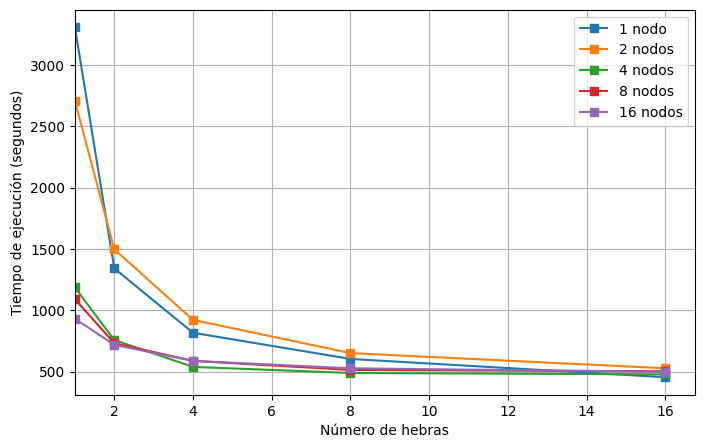
\includegraphics[width=0.8\textwidth]{imagenes/cap5/thread_sweep_windows_docker_time.png}
    \caption{Tiempo de ejecución en función del número de hebras en contenedores \textit{Docker} de Windows (CPU).}
    \label{fig:thread_sweep_windows_docker_time}
\end{figure}

En la tabla \ref{tab:thread_sweep_windows_docker_time} se presentan los tiempos de ejecución y la reducción porcentual respecto a una hebra.

\begin{table}[ht]
    \centering
    \begin{tabular}{|c|c|c|c|}
        \hline
        \textbf{Procesos} & \textbf{Hebras} & \textbf{Tiempo (s)} & \textbf{$\Delta$\% vs 1 hebra} \\
        \hline
        1.00              & 1.00            & 3308.08             & 0.00                           \\
        1.00              & 2.00            & 1341.41             & -59.45                         \\
        1.00              & 4.00            & 816.06              & -75.33                         \\
        1.00              & 8.00            & 602.60              & -81.78                         \\
        1.00              & 16.00           & 453.44              & -86.29                         \\
        2.00              & 1.00            & 2708.91             & 0.00                           \\
        2.00              & 2.00            & 1497.01             & -44.74                         \\
        2.00              & 4.00            & 921.23              & -65.99                         \\
        2.00              & 8.00            & 650.28              & -75.99                         \\
        2.00              & 16.00           & 526.23              & -80.57                         \\
        4.00              & 1.00            & 1185.46             & 0.00                           \\
        4.00              & 2.00            & 757.13              & -36.13                         \\
        4.00              & 4.00            & 537.45              & -54.66                         \\
        4.00              & 8.00            & 488.12              & -58.82                         \\
        4.00              & 16.00           & 476.64              & -59.79                         \\
        8.00              & 1.00            & 1090.62             & 0.00                           \\
        8.00              & 2.00            & 731.08              & -32.97                         \\
        8.00              & 4.00            & 586.55              & -46.22                         \\
        8.00              & 8.00            & 512.87              & -52.97                         \\
        8.00              & 16.00           & 501.93              & -53.98                         \\
        16.00             & 1.00            & 930.79              & 0.00                           \\
        16.00             & 2.00            & 717.75              & -22.89                         \\
        16.00             & 4.00            & 586.84              & -36.95                         \\
        16.00             & 8.00            & 526.20              & -43.47                         \\
        16.00             & 16.00           & 497.09              & -46.60                         \\
        \hline
    \end{tabular}
    \caption{Tiempos de ejecución y reducción porcentual respecto a una hebra para distintas combinaciones de procesos y hebras en contenedores \textit{Docker} de Windows (CPU).}
    \label{tab:thread_sweep_windows_docker_time}
\end{table}

La tabla muestra los tiempos de ejecución y la reducción porcentual respecto a una hebra para distintas combinaciones de procesos y hebras en contenedores \textit{Docker} de Windows utilizando CPU. Se observa que, en configuraciones monoproceso, el incremento del número de hebras produce una reducción muy significativa del tiempo de ejecución, alcanzando una disminución del 86.29\% con dieciséis hebras respecto a la ejecución secuencial. El mayor beneficio se obtiene al pasar de una a dos hebras (-59.45\%) y de dos a cuatro hebras (-15.88\% adicional), lo que indica una excelente escalabilidad inicial. A medida que se incrementa el número de procesos, la reducción porcentual respecto a una hebra disminuye progresivamente y el beneficio de añadir más hebras es cada vez menor. Por ejemplo, con dieciséis procesos y dieciséis hebras, la reducción es del 46.60\%, notablemente inferior a la obtenida en el caso monoproceso. Además, en configuraciones con muchos procesos, el incremento de hebras sigue aportando mejoras, pero estas son más limitadas, lo que sugiere que la sobrecarga de coordinación y la gestión de recursos entre contenedores penalizan la eficiencia del paralelismo. En conjunto, \textit{Docker} sobre Windows permite un aprovechamiento eficiente del paralelismo en configuraciones monoproceso, pero la eficiencia disminuye al aumentar el número de procesos, especialmente cuando se incrementa la complejidad de la comunicación y la gestión de procesos distribuidos.

En la figura \ref{fig:thread_sweep_windows_podman_time} se muestra el tiempo de ejecución para la configuración de CPU en un entorno con contenedores de \textit{Podman}.

\begin{figure}[H]
    \centering
    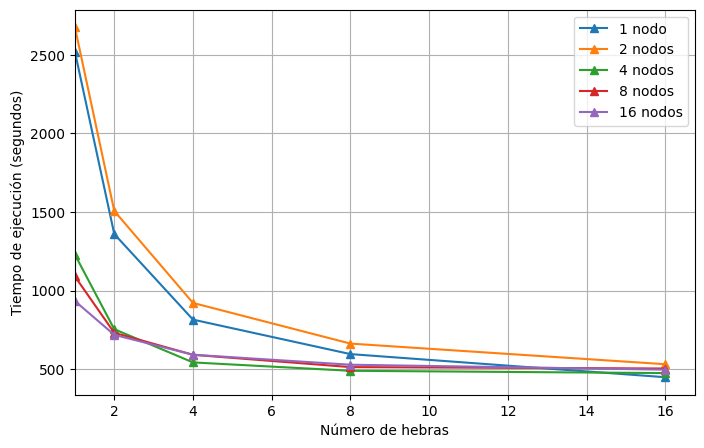
\includegraphics[width=0.8\textwidth]{imagenes/cap5/thread_sweep_windows_podman_time.png}
    \caption{Tiempo de ejecución en función del número de hebras en contenedores de \textit{Podman} (CPU).}
    \label{fig:thread_sweep_windows_podman_time}
\end{figure}

En la tabla \ref{tab:thread_sweep_windows_podman_time} se presentan los tiempos de ejecución y la reducción porcentual respecto a una hebra.

\begin{table}[ht]
    \centering
    \begin{tabular}{|c|c|c|c|}
        \hline
        \textbf{Procesos} & \textbf{Hebras} & \textbf{Tiempo (s)} & \textbf{$\Delta$\% vs 1 hebra} \\
        \hline
        1.00              & 1.00            & 2520.21             & 0.00                           \\
        1.00              & 2.00            & 1359.69             & -46.05                         \\
        1.00              & 4.00            & 815.04              & -67.66                         \\
        1.00              & 8.00            & 595.54              & -76.37                         \\
        1.00              & 16.00           & 448.43              & -82.21                         \\
        2.00              & 1.00            & 2675.94             & 0.00                           \\
        2.00              & 2.00            & 1506.57             & -43.70                         \\
        2.00              & 4.00            & 921.20              & -65.57                         \\
        2.00              & 8.00            & 662.40              & -75.25                         \\
        2.00              & 16.00           & 531.13              & -80.15                         \\
        4.00              & 1.00            & 1228.59             & 0.00                           \\
        4.00              & 2.00            & 754.03              & -38.63                         \\
        4.00              & 4.00            & 542.63              & -55.83                         \\
        4.00              & 8.00            & 489.36              & -60.17                         \\
        4.00              & 16.00           & 474.74              & -61.36                         \\
        8.00              & 1.00            & 1089.75             & 0.00                           \\
        8.00              & 2.00            & 731.20              & -32.90                         \\
        8.00              & 4.00            & 591.11              & -45.76                         \\
        8.00              & 8.00            & 512.87              & -52.94                         \\
        8.00              & 16.00           & 503.82              & -53.77                         \\
        16.00             & 1.00            & 933.45              & 0.00                           \\
        16.00             & 2.00            & 718.20              & -23.06                         \\
        16.00             & 4.00            & 591.53              & -36.63                         \\
        16.00             & 8.00            & 527.98              & -43.44                         \\
        16.00             & 16.00           & 496.62              & -46.80                         \\
        \hline
    \end{tabular}
    \caption{Tiempos de ejecución y reducción porcentual respecto a una hebra para distintas combinaciones de procesos y hebras en contenedores de \textit{Podman} sobre Windows (CPU).}
    \label{tab:thread_sweep_windows_podman_time}
\end{table}

La tabla muestra los tiempos de ejecución y la reducción porcentual respecto a una hebra para distintas combinaciones de procesos y hebras en contenedores de \textit{Podman} sobre Windows (CPU). Se observa que, en configuraciones monoproceso, el incremento del número de hebras produce una reducción significativa del tiempo de ejecución, alcanzando una disminución del 82.21\% con 16 hebras respecto a la ejecución secuencial. El mayor beneficio se obtiene al pasar de 1 a 2 hebras (-46.05\%) y de 2 a 4 hebras (-21.61\% adicional), lo que indica una buena escalabilidad inicial. A medida que se incrementa el número de procesos, la reducción porcentual respecto a una hebra disminuye progresivamente y el beneficio de añadir más hebras es cada vez menor. Por ejemplo, con 16 procesos y 16 hebras, la reducción es del 46.80\%, notablemente inferior a la obtenida en el caso monoproceso. Además, en configuraciones con muchos procesos, el incremento de hebras sigue aportando mejoras, pero estas son más limitadas, lo que sugiere que la sobrecarga de coordinación y la gestión de recursos entre contenedores penalizan la eficiencia del paralelismo. En conjunto, \textit{Podman} sobre Windows permite un aprovechamiento eficiente del paralelismo en configuraciones monoproceso, pero la eficiencia disminuye al aumentar el número de procesos, especialmente cuando se incrementa la complejidad de la comunicación y la gestión de procesos distribuidos.

\subsubsection{CPU + GPU}

\subsection{Ejecución en contenedores de Mac}
\subsubsection{CPU}

En la figura \ref{fig:thread_sweep_mac_docker_time} se muestra el tiempo de ejecución para la configuración de CPU en un entorno con contenedores de Mac.

\begin{figure}[H]
    \centering
    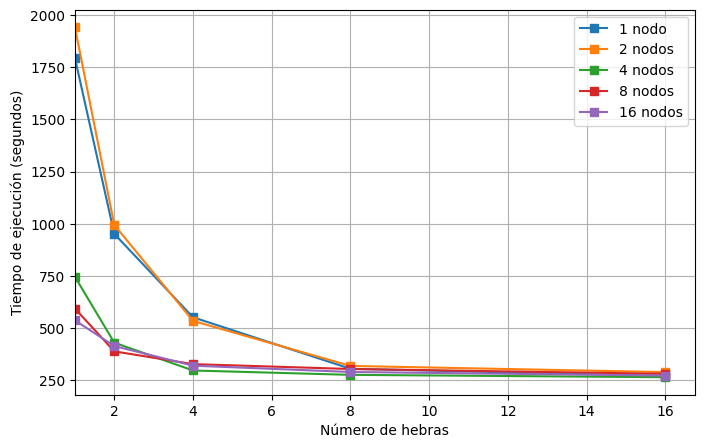
\includegraphics[width=0.8\textwidth]{imagenes/cap5/thread_sweep_mac_docker_time.png}
    \caption{Tiempo de ejecución en función del número de hebras en contenedores \textit{Docker} de Mac (CPU).}
    \label{fig:thread_sweep_mac_docker_time}
\end{figure}

En la tabla \ref{tab:thread_sweep_mac_docker_time} se presentan los tiempos de ejecución y la reducción porcentual respecto a una hebra.

\begin{table}[ht]
    \centering
    \begin{tabular}{|c|c|c|c|}
        \hline
        \textbf{Procesos} & \textbf{Hebras} & \textbf{Tiempo (s)} & \textbf{$\Delta$\% vs 1 hebra} \\
        \hline
        1.00              & 1.00            & 1794.98             & 0.00                           \\
        1.00              & 2.00            & 951.56              & -46.99                         \\
        1.00              & 4.00            & 551.41              & -69.28                         \\
        1.00              & 8.00            & 304.35              & -83.04                         \\
        1.00              & 16.00           & 270.25              & -84.94                         \\
        2.00              & 1.00            & 1942.42             & 0.00                           \\
        2.00              & 2.00            & 994.15              & -48.82                         \\
        2.00              & 4.00            & 534.05              & -72.51                         \\
        2.00              & 8.00            & 318.04              & -83.63                         \\
        2.00              & 16.00           & 288.41              & -85.15                         \\
        4.00              & 1.00            & 745.84              & 0.00                           \\
        4.00              & 2.00            & 429.82              & -42.37                         \\
        4.00              & 4.00            & 296.17              & -60.29                         \\
        4.00              & 8.00            & 275.30              & -63.09                         \\
        4.00              & 16.00           & 263.92              & -64.61                         \\
        8.00              & 1.00            & 593.47              & 0.00                           \\
        8.00              & 2.00            & 388.01              & -34.62                         \\
        8.00              & 4.00            & 326.75              & -44.94                         \\
        8.00              & 8.00            & 303.35              & -48.89                         \\
        8.00              & 16.00           & 280.15              & -52.79                         \\
        16.00             & 1.00            & 536.60              & 0.00                           \\
        16.00             & 2.00            & 413.59              & -22.92                         \\
        16.00             & 4.00            & 319.30              & -40.50                         \\
        16.00             & 8.00            & 289.00              & -46.14                         \\
        16.00             & 16.00           & 271.75              & -49.36                         \\
        \hline
    \end{tabular}
    \caption{Tiempos de ejecución y reducción porcentual respecto a una hebra para distintas combinaciones de procesos y hebras en contenedores \textit{Docker} de Mac (CPU).}
    \label{tab:thread_sweep_mac_docker_time}
\end{table}

La tabla muestra los tiempos de ejecución y la reducción porcentual respecto a una hebra para distintas combinaciones de procesos y hebras en contenedores \textit{Docker} de Mac (CPU). Se observa que, en configuraciones monoproceso, el incremento del número de hebras produce una reducción muy significativa del tiempo de ejecución, alcanzando una disminución del 84.94\% con 16 hebras respecto a la ejecución secuencial. El mayor beneficio se obtiene al pasar de 1 a 2 hebras (-46.99\%) y de 2 a 4 hebras (-22.29\% adicional), lo que indica una buena escalabilidad inicial. A partir de 8 hebras, la mejora se estabiliza y el beneficio adicional es menor, lo que sugiere que el paralelismo óptimo se sitúa en torno a 8 hebras.

Al aumentar el número de procesos, la reducción porcentual respecto a una hebra sigue una tendencia similar: con 2 y 4 procesos se mantienen reducciones superiores al 60\%, pero a partir de 8 y 16 procesos las mejoras adicionales son más limitadas. Además, en algunos casos, como al pasar de 1 a 2 procesos, se observa un ligero aumento en el tiempo de ejecución, probablemente debido a la sobrecarga de coordinación entre procesos en el entorno de \textit{Docker} sobre Mac.

En resumen, \textit{Docker} sobre Mac permite un aprovechamiento eficiente del paralelismo hasta cierto punto, siendo recomendable utilizar hasta 8 hebras por proceso para maximizar el rendimiento. Aumentar el número de procesos y hebras más allá de ese valor aporta mejoras cada vez menores, debido a la sobrecarga de coordinación y a las limitaciones propias del entorno.

En la figura \ref{fig:thread_sweep_mac_podman_time} se muestra el tiempo de ejecución para la configuración de CPU en un entorno con contenedores de \textit{Podman}.

\begin{figure}[H]
    \centering
    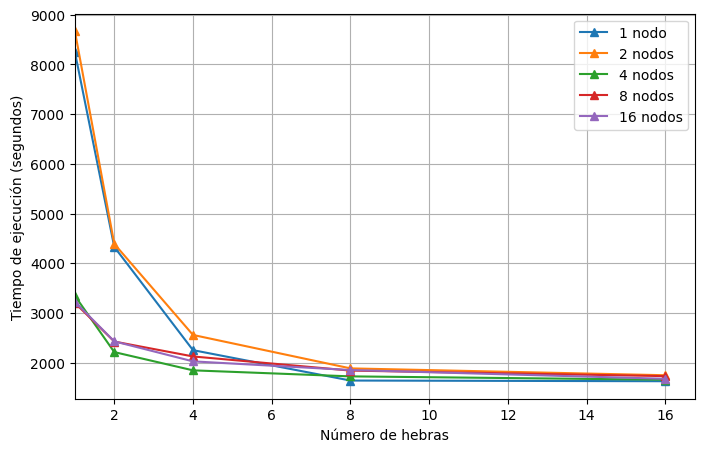
\includegraphics[width=0.8\textwidth]{imagenes/cap5/thread_sweep_mac_podman_time.png}
    \caption{Tiempo de ejecución en función del número de hebras en contenedores de \textit{Podman} (CPU).}
    \label{fig:thread_sweep_mac_podman_time}
\end{figure}

En la tabla \ref{tab:thread_sweep_mac_podman_time} se presentan los tiempos de ejecución y la reducción porcentual respecto a una hebra.

\begin{table}[ht]
    \centering
    \begin{tabular}{|c|c|c|c|}
        \hline
        \textbf{Procesos} & \textbf{Hebras} & \textbf{Tiempo (s)} & \textbf{$\Delta$\% vs 1 hebra} \\
        \hline
        1.00              & 1.00            & 8247.00             & 0.00                           \\
        1.00              & 2.00            & 4328.00             & -47.52                         \\
        1.00              & 4.00            & 2250.20             & -72.71                         \\
        1.00              & 8.00            & 1638.79             & -80.13                         \\
        1.00              & 16.00           & 1625.19             & -80.29                         \\
        2.00              & 1.00            & 8668.00             & 0.00                           \\
        2.00              & 2.00            & 4389.00             & -49.37                         \\
        2.00              & 4.00            & 2556.33             & -70.51                         \\
        2.00              & 8.00            & 1883.55             & -78.27                         \\
        2.00              & 16.00           & 1745.53             & -79.86                         \\
        4.00              & 1.00            & 3343.15             & 0.00                           \\
        4.00              & 2.00            & 2211.26             & -33.86                         \\
        4.00              & 4.00            & 1844.13             & -44.84                         \\
        4.00              & 8.00            & 1722.73             & -48.47                         \\
        4.00              & 16.00           & 1655.26             & -50.49                         \\
        8.00              & 1.00            & 3201.07             & 0.00                           \\
        8.00              & 2.00            & 2423.60             & -24.29                         \\
        8.00              & 4.00            & 2123.61             & -33.66                         \\
        8.00              & 8.00            & 1839.23             & -42.54                         \\
        8.00              & 16.00           & 1727.69             & -46.03                         \\
        16.00             & 1.00            & 3223.98             & 0.00                           \\
        16.00             & 2.00            & 2427.40             & -24.71                         \\
        16.00             & 4.00            & 2024.70             & -37.20                         \\
        16.00             & 8.00            & 1850.36             & -42.61                         \\
        16.00             & 16.00           & 1674.10             & -48.07                         \\
        \hline
    \end{tabular}
    \caption{Tiempos de ejecución y reducción porcentual respecto a una hebra para distintas combinaciones de procesos y hebras en contenedores de \textit{Podman} sobre Mac (CPU).}
    \label{tab:thread_sweep_mac_podman_time}
\end{table}

La tabla muestra los tiempos de ejecución y la reducción porcentual respecto a una hebra para distintas combinaciones de procesos y hebras en contenedores de \textit{Podman} sobre Mac (CPU). Se observa que, en configuraciones monoproceso, el incremento del número de hebras produce una reducción significativa del tiempo de ejecución, alcanzando una disminución del 80.29\% con 16 hebras respecto a la ejecución secuencial. El mayor beneficio se obtiene al pasar de 1 a 2 hebras (-47.52\%) y de 2 a 4 hebras (-25.19\% adicional), lo que indica una buena escalabilidad inicial. Sin embargo, a partir de 8 hebras, la mejora se estabiliza y el beneficio adicional es mínimo, sugiriendo que el paralelismo óptimo se sitúa en torno a 8 hebras.

Al aumentar el número de procesos, la reducción porcentual respecto a una hebra disminuye progresivamente. Por ejemplo, con 16 procesos y 16 hebras, la reducción es del 48.07\%, notablemente inferior a la obtenida en el caso monoproceso. Además, en configuraciones con muchos procesos, el incremento de hebras aporta mejoras cada vez más limitadas, lo que sugiere que la sobrecarga de coordinación y la gestión de recursos entre contenedores penalizan la eficiencia del paralelismo.

En resumen, \textit{Podman} sobre Mac permite un aprovechamiento eficiente del paralelismo en configuraciones monoproceso, pero la eficiencia disminuye al aumentar el número de procesos, especialmente cuando se incrementa la complejidad de la comunicación y la gestión de procesos distribuidos. El punto óptimo de eficiencia se alcanza alrededor de 8 hebras por proceso.